% ============================================================
%  7. DESARROLLO (SECCIÓN APLICATIVA: CRISP-DM)   (guía, 2.7 / Anexo A)
%  ------------------------------------------------------------
%  Aquí se documenta la EJECUCIÓN REAL del proyecto, organizada
%  según las seis fases de CRISP-DM.
%  Regla transversal de la guía: justificar decisiones, no
%  enumerar comandos ni librerías; interpretar resultados, no
%  solo mostrarlos.
%
%  Este archivo solo abre el capítulo e incluye las seis fases,
%  una por archivo, para poder trabajar sobre una sin tocar las
%  demás. Se incluyen con \input y no con \include porque las
%  fases son SECCIONES del mismo capítulo y no deben empezar en
%  página nueva.
% ============================================================
\chapter{Desarrollo (sección aplicativa: CRISP-DM)}
\label{cap:desarrollo}

% ============================================================
%  7.1. COMPRENSIÓN DEL NEGOCIO  -- parte del capítulo 7
%  ------------------------------------------------------------
%  Guía 2.7.1: (1) contexto operativo o institucional,
%  (2) traducción de la necesidad, (3) resultado esperado y
%  criterio de utilidad, (4) enlace con lo ya escrito.
%  No es "Comprensión de los datos" (fuentes, variables, EDA):
%  eso va en 08_02.
%  Fuente de verdad: trufi-data-science (EXPLICATIVO.md,
%  config.py, resultados/<fase>/metricas.json).
% ============================================================
\section{Comprensión del negocio}
\label{sec:comprension-negocio}

Esta primera fase de CRISP-DM define para quién se trabaja, qué decisión se quiere apoyar y
cómo se reconocerá que el resultado sirve. No trata todavía de los datos, que se describen
en la sección~\ref{sec:comprension-datos}, sino del proceso real de la organización y del
modo en que su necesidad se convierte en un problema que la Ciencia de Datos puede
abordar.

\subsection{Contexto operativo e institucional}
\label{sec:contexto-operativo}

Trufi Association es una organización sin fines de lucro que mantiene Trufi App, un
planificador de viajes para el transporte público del eje metropolitano de Cochabamba.
Como la mayor parte de ese transporte opera bajo la modalidad de paratránsito, sin
horarios ni paradas oficiales publicadas (sección~\ref{subsec:paratransito}), la
información que ofrece la aplicación no proviene de los operadores, sino de un
relevamiento colaborativo. El proceso real tiene cuatro pasos:
\begin{enumerate}
  \item Un grupo de voluntarios recorre una línea de micro o trufi.
  \item Los voluntarios registran su trayecto en OpenStreetMap
        (sección~\ref{subsec:cartografia-colaborativa}).
  \item El trazado se verifica con los operadores o en terreno.
  \item El trazado se convierte al formato GTFS (sección~\ref{subsec:gtfs}), que es el que
        consume el planificador de la aplicación.
\end{enumerate}
El feed resultante, empleado en este trabajo, describe 141 líneas de 43 operadores.

Cada jornada de mapeo consume desplazamientos, tiempo de edición y coordinación entre
personas que colaboran de forma voluntaria. Por eso la capacidad de la organización es
limitada, y cada jornada debe dirigirse a alguna zona concreta del territorio. Hoy esa
elección descansa en el conocimiento acumulado del equipo y en observaciones informales.
Al mismo tiempo, la aplicación genera de forma pasiva un registro de cada consulta de ruta
que realizan sus usuarios, con origen, destino, hora e identificador anónimo de
instalación. Ese registro abarca casi dos años (septiembre de 2022 a junio de 2024) y más
de 1,9~millones de consultas, pero no forma parte del proceso con el que se decide dónde
mapear. El punto de partida del proyecto es esa desconexión entre un proceso operativo que
necesita priorizar y un registro de uso que no se aprovecha para hacerlo.

\subsection{Traducción de la necesidad a un problema de Ciencia de Datos}
\label{sec:traduccion-necesidad}

La necesidad de la organización se expresa en términos operativos: \emph{¿a qué zonas
conviene enviar primero a los voluntarios?} Esa pregunta no puede responderse contando
consultas, porque un conteo bajo es ambiguo (sección~\ref{sec:descripcion-problema}).
Puede tratarse de una zona con poca población, o de una zona donde la aplicación no ofrece
información útil y, por eso, casi nadie la consulta. Para separar ambas situaciones hace
falta una referencia: cuántas consultas \emph{cabría esperar} en cada zona si se
comportara como las zonas comparables.

Con esa idea, la necesidad se traduce en un problema analítico de dos pasos:

\begin{enumerate}
  \item \textbf{Estimar el conteo esperado de consultas por zona.} Es un problema de
    regresión sobre datos de conteo (sección~\ref{subsec:datos-conteo}). La variable a
    estimar es el total de consultas originadas en cada zona H3 de resolución~8 durante el
    período, y la población residente actúa como \emph{exposición}: a igualdad de
    condiciones, una zona con el doble de habitantes debería generar el doble de consultas.
    Lo esperado se estima con información que no depende de la red mapeada: la población y
    la localización de la zona.
  \item \textbf{Comparar lo observado con lo esperado.} La diferencia entre ambos,
    expresada en una escala comparable entre zonas grandes y pequeñas, se denomina
    \emph{brecha} (sección~\ref{subsec:observado-esperado}). Una brecha negativa indica que
    la zona consulta menos de lo que cabría esperar por su población y su entorno. Esa
    señal, contrastada después con la cobertura de la red mapeada, orienta la revisión en
    terreno.
\end{enumerate}

Conviene precisar lo que el problema \emph{no} es. No es un pronóstico temporal, porque no
se predice cuántas consultas habrá la semana próxima, sino cuántas corresponden a cada zona
en el período observado. Tampoco es una clasificación de zonas en ``bien'' o ``mal''
mapeadas, porque no existe una etiqueta verificada de cobertura real con la cual entrenar
un clasificador. La cobertura de la red mapeada se excluye deliberadamente del cálculo de
lo esperado: si se incluyera, el modelo aprendería que las zonas sin rutas consultan poco y
les asignaría una expectativa baja, con lo que la brecha que se busca detectar desaparecería
por construcción.

\subsection{Resultado esperado y criterio de utilidad}
\label{sec:criterio-utilidad}

El resultado que se espera entregar a Trufi Association no es ``un modelo'', sino tres
productos que puedan usarse sin conocimientos de programación:
\begin{itemize}
  \item un archivo con el valor observado, el esperado y la brecha de cada zona;
  \item un mapa interactivo de la brecha;
  \item una lista corta de veinte zonas priorizadas para la revisión en terreno.
\end{itemize}
La mejora que se persigue es operativa: sustituir la elección informal entre más de mil
zonas por una lista corta, ordenada y justificada con datos.

Para que esa lista sea confiable, la técnica que produce el esperado debe cumplir criterios
medibles, fijados antes de ajustar cualquier modelo. La técnica se elegirá entre siete
alternativas de complejidad creciente. Sus códigos (B0 a B3 y M1 a M3) se explican en la
sección~\ref{sec:seleccion-algoritmos}. La tabla~\ref{tab:criterios-utilidad} resume los
criterios, cómo se mide cada uno y qué pregunta de la organización responde.

\begin{table}[H]
  \centering
  \caption{Criterios de utilidad declarados antes de modelar}
  \label{tab:criterios-utilidad}
  \interlineadoSimple
  \small
  \begin{tabularx}{\textwidth}{@{}L{0.23\textwidth}L{0.33\textwidth}Y@{}}
    \toprule
    \textbf{Criterio} & \textbf{Cómo se mide} & \textbf{Pregunta que responde} \\
    \midrule
    Supera al punto de referencia inicial & $D^2$ frente a la tasa global en zonas no vistas, mayor que cero & ¿El contexto territorial aporta algo más que la población? \\
    Ordena bien las zonas & Correlación de Spearman entre observado y esperado & ¿Las zonas que más consultan quedan arriba? \\
    Está calibrada & Suma de lo esperado dividida entre suma de lo observado, cercana a 1 & ¿El volumen total estimado es realista? \\
    Es estable & Índice de Jaccard del top-20 ante variaciones razonables & ¿La lista cambia si se modifica un supuesto menor? \\
    Es accionable & Número de zonas que el equipo debe revisar & ¿Se reduce el trabajo de decisión? \\
    \bottomrule
  \end{tabularx}
  \fuente{Elaboración propia. Las métricas se definen en la sección~\ref{sec:metricas}; los
  valores obtenidos se presentan en la sección~\ref{sec:evaluacion-resultados}.}
\end{table}

A estos criterios se suman dos reglas de protocolo, también declaradas de antemano. La
primera es que la técnica se elige con una regla escrita antes de ver los resultados, y no
por ser la primera que se probó ni la de menor error aparente
(sección~\ref{sec:regla-seleccion}). La segunda es que el conjunto de prueba se evalúa una
sola vez, al final.

La señal definitiva de utilidad, sin embargo, no es estadística. Sería la proporción de
zonas visitadas en las que los voluntarios encuentran rutas sin mapear. Esa verificación
en terreno excede el alcance de la materia (capítulo~\ref{cap:alcance}) y no se ha
realizado. Para que pueda medirse en cuanto empiecen las visitas, el archivo
\var{zonas_prioritarias.csv} incluye dos columnas de registro:
\begin{itemize}
  \item \var{field_result}, que registra el resultado de la visita con una de cuatro
        categorías: \var{ruta_no_mapeada}, \var{ruta_mapeada_correcta}, \var{sin_transporte}
        o \var{sin_visitar}. Esta última viene precargada en las veinte zonas.
  \item \var{field_notes}, que queda libre para observaciones.
\end{itemize}
El protocolo correspondiente se describe en la sección~\ref{sec:productos-despliegue}.

\subsection{Enlace con el problema, el alcance y los objetivos}
\label{sec:enlace-objetivos}

Esta fase concreta en términos operativos lo que los capítulos anteriores plantearon en
términos de investigación:
\begin{itemize}
  \item La ambigüedad del conteo descrita en el capítulo~\ref{cap:problema} se resuelve con
        la comparación entre lo observado y lo esperado.
  \item Las exclusiones del capítulo~\ref{cap:alcance} (sin pronóstico temporal, sin datos
        externos ni imputación de semanas faltantes, sin despliegue en producción) delimitan
        las técnicas admisibles y el tipo de entrega.
  \item Cada objetivo específico del capítulo~\ref{cap:objetivos} corresponde a una o dos
        fases de CRISP-DM y deja una evidencia verificable en el repositorio del proyecto,
        como se muestra en la tabla~\ref{tab:trazabilidad-oe}.
\end{itemize}

\begin{table}[H]
  \centering
  \caption{Correspondencia entre objetivos específicos, fases y evidencias}
  \label{tab:trazabilidad-oe}
  \interlineadoSimple
  \small
  \begin{tabularx}{\textwidth}{@{}L{0.07\textwidth}L{0.25\textwidth}L{0.17\textwidth}Y@{}}
    \toprule
    \textbf{OE} & \textbf{Fase y notebook} & \textbf{Sección} & \textbf{Evidencia principal} \\
    \midrule
    OE1 & Comprensión de los datos (\var{01_eda}); preparación (\var{02_preprocesamiento}, \var{03_feature_engineering}) & \ref{sec:comprension-datos} y \ref{sec:preparacion-datos} & Tabla de 1.628 zonas con consultas, población y cobertura; \var{metricas.json} de las tres fases \\
    OE2 & Preparación (reserva de prueba, \var{03_feature_engineering}); modelado (\var{04_modelado}) & \ref{sec:conjuntos-entrenamiento-prueba} y \ref{sec:modelado} & Bloques de prueba (\var{test_blocks.csv}); comparación de siete técnicas (\var{cv_resumen.csv}); regla de selección (\var{regla_seleccion.csv}) \\
    OE3 & Evaluación (\var{05_evaluacion}) & \ref{sec:evaluacion-resultados} & Métricas de prueba, brecha por zona, contraste con la cobertura y sensibilidad \\
    OE4 & Despliegue como propuesta (\var{06_propuesta}) & \ref{sec:despliegue} & Predicciones por zona, lista de veinte zonas prioritarias, mapa interactivo y procedimiento de actualización \\
    \bottomrule
  \end{tabularx}
  \fuente{Elaboración propia, a partir de la estructura del repositorio
  \var{trufi-data-science} (carpetas \var{notebooks/} y \var{resultados/}).}
\end{table}

La figura~\ref{fig:flujo-crisp-proyecto} muestra cómo se instanciaron las seis fases de
CRISP-DM en el proyecto. Cada fase de datos corresponde a un notebook que lee lo que dejó
la anterior, regenera sus salidas y termina con verificaciones automáticas de sus propias
cifras.

El carácter iterativo de la metodología (sección~\ref{sec:crisp-dm}) se manifestó en dos
retornos concretos a esta fase, señalados con flechas discontinuas en la figura:
\begin{itemize}
  \item El análisis exploratorio fijó la delimitación operativa del área de estudio, que
        el capítulo~\ref{cap:alcance} había dejado abierta a propósito
        (sección~\ref{sec:area-estudio}).
  \item La evaluación mostró que la lista de zonas con mayor brecha estaba formada casi por
        completo por zonas ya cubiertas por la red mapeada
        (sección~\ref{sec:interpretacion-resultados}). Como en esas zonas mapear no aporta,
        se precisó el criterio de utilidad: la lista priorizada se restringe a zonas sin
        trazado cercano.
\end{itemize}
La técnica elegida no se modificó por ese cambio. Ambas decisiones quedan documentadas
como tales, y no se presentan como parte del diseño original.

\begin{figure}[H]
  \centering
  \caption{Flujo CRISP-DM del proyecto: fases, notebooks y objetivos específicos}
  \label{fig:flujo-crisp-proyecto}
  \begin{tikzpicture}[
      font=\small,
      fase/.style={draw, rounded corners=3pt, fill=gray!8, align=center,
                   text width=4.0cm, minimum height=2.1cm, inner sep=3pt},
      flecha/.style={-{Stealth[length=2.5mm]}, thick},
      retorno/.style={-{Stealth[length=2.5mm]}, thick, dashed, gray!70!black},
      node distance=0.9cm and 0.45cm]
    \node[fase] (f1) {\textbf{1. Comprensión\\del negocio}\\[2pt] sección~\ref{sec:comprension-negocio}};
    \node[fase, right=of f1] (f2) {\textbf{2. Comprensión\\de los datos}\\[2pt] {\footnotesize\texttt{01\_eda}}\\ OE1};
    \node[fase, right=of f2, text width=5.0cm] (f3) {\textbf{3. Preparación\\de los datos}\\[2pt] {\footnotesize\texttt{02\_preprocesamiento}}\\ {\footnotesize\texttt{03\_feature\_engineering}}\\ OE1 y OE2};
    \node[fase, below=1.4cm of f3, text width=5.0cm] (f4) {\textbf{4. Modelado}\\[2pt] {\footnotesize\texttt{04\_modelado}}\\ OE2};
    \node[fase, left=of f4] (f5) {\textbf{5. Evaluación}\\[2pt] {\footnotesize\texttt{05\_evaluacion}}\\ OE3};
    \node[fase, left=of f5] (f6) {\textbf{6. Despliegue}\\ (propuesta)\\[2pt] {\footnotesize\texttt{06\_propuesta}}\\ OE4};
    \draw[flecha] (f1) -- (f2);
    \draw[flecha] (f2) -- (f3);
    \draw[flecha] (f3) -- (f4);
    \draw[flecha] (f4) -- (f5);
    \draw[flecha] (f5) -- (f6);
    \draw[retorno] (f2.north) to[bend right=25]
      node[above, font=\footnotesize, text=black] {delimitación del área} (f1.north);
    \draw[retorno] ($(f5.north west)+(0.5,0)$) --
      node[right, pos=0.5, font=\footnotesize, text=black] {regla de priorización}
      ($(f1.south east)+(-0.5,0)$);
  \end{tikzpicture}
  \fuente{Elaboración propia. Las flechas discontinuas señalan los dos retornos documentados
  a la comprensión del negocio.}
\end{figure}

% ============================================================
%  7.2. COMPRENSIÓN DE LOS DATOS  -- parte del capítulo 7
%  ------------------------------------------------------------
%  Guía 2.7.2: (1) fuentes, (2) variables y diccionario,
%  (3) EDA, (4) distribución, calidad, faltantes, atípicos y
%  relaciones, (5) gráficos y estadísticas, (6) hallazgos que
%  influyen en la preparación y el modelado.
%  Notebook: trufi-data-science/notebooks/01_eda.ipynb
%  Cifras:   resultados/01_eda/metricas.json y CSV de la carpeta.
% ============================================================
\section{Comprensión de los datos}
\label{sec:comprension-datos}

Esta fase examina las tres fuentes del proyecto antes de transformarlas. Tiene tres
propósitos:
\begin{itemize}
  \item medir su calidad;
  \item describir la variable que se va a estimar;
  \item fijar, con evidencia, los criterios que aplicará la preparación de los datos.
\end{itemize}
Se ejecuta en el notebook \var{01_eda}, que lee únicamente \var{data/raw/} y no escribe en
\var{data/}, de modo que ninguna decisión de limpieza se aplica todavía: solo se mide su
efecto. Las cifras de esta sección provienen de \var{resultados/01_eda/metricas.json} y de
los archivos CSV de la misma carpeta.

\subsection{Fuentes de datos}
\label{sec:fuentes-datos}

El proyecto emplea tres fuentes, todas conservadas sin modificar en \var{data/raw/}. La
tabla~\ref{tab:fuentes-datos} resume su origen, su contenido y las condiciones en que se
obtuvieron.

\begin{table}[H]
  \centering
  \caption{Fuentes de datos del proyecto}
  \label{tab:fuentes-datos}
  \interlineadoSimple
  \small
  \begin{tabularx}{\textwidth}{@{}L{0.20\textwidth}L{0.22\textwidth}Y@{}}
    \toprule
    \textbf{Fuente} & \textbf{Productor y obtención} & \textbf{Contenido y cobertura} \\
    \midrule
    Consultas de ``Trufi App'' & Trufi Association; exportaciones semanales del registro de la aplicación, entregadas para este trabajo & 85 archivos CSV que cubren 84 semanas ISO con datos, del 12-09-2022 al 09-06-2024 (la semana del 26-12-2022 al 01-01-2023 viene partida en dos archivos, sin filas repetidas); 1.927.675 consultas con origen, destino, fecha y hora, identificador anónimo de instalación, distancia y municipio de origen y destino \\
    Kontur Population, edición 2023-11-01 & Kontur; conjunto abierto descargado en formato GeoPackage comprimido & Población residente estimada por celda H3 de resolución~8 para toda Bolivia: 145.929 celdas y 12.431.735 habitantes (sección~\ref{subsec:kontur}) \\
    Feed GTFS de Trufi Cochabamba & Trufi Association; generado a partir del mapeo colaborativo en OpenStreetMap & 11 tablas: 43 operadores, 141 líneas y 626 recorridos con su trazado (una línea puede tener varios recorridos, por ejemplo ida y vuelta), 22.320 paradas y frecuencias; vigencia declarada desde el 01-01-2024 \\
    \bottomrule
  \end{tabularx}
  \fuente{Elaboración propia, a partir de \var{01_eda} (secciones 2 y 7) y
  \var{resultados/01_eda/metricas.json}.}
\end{table}

Las tres fuentes cumplen funciones distintas, y conviene fijarlas desde el inicio porque
condicionan todo lo que sigue:
\begin{itemize}
  \item Las \textbf{consultas} producen la variable objetivo, que es el número de consultas
        originadas en cada zona.
  \item \textbf{Kontur} aporta la exposición (la población residente) y las variables de
        entorno poblacional.
  \item El \textbf{GTFS} describe la red mapeada, y en este proyecto se usa solo para
        \emph{interpretar} la brecha, nunca como predictor (sección~\ref{sec:traduccion-necesidad}).
\end{itemize}
Una consulta es una búsqueda de ruta en la aplicación, no un viaje realizado: refleja la
necesidad de información de quienes usan ``Trufi App'', no la movilidad de toda la población
(sección~\ref{subsec:consultas-senal}).

\subsection{Variables y diccionario de datos}
\label{sec:diccionario-datos}

Las exportaciones de consultas llegaron en dos esquemas:
\begin{itemize}
  \item El \emph{lote original} reúne 79 archivos, desde 2022-W37 hasta 2024-W10. Tiene 13
        columnas en codificación UTF-8 y nombres temporales en español (\var{hora},
        \var{dia_de_semana}, \var{dia_de_mes}, \var{fin_de_semana}).
  \item El \emph{lote 2024} reúne 6 archivos, desde 2024-W18 hasta 2024-W23. Tiene 15
        columnas en codificación Latin-1, nombres temporales en inglés y dos campos nuevos
        (\var{year_week_number} y \var{time_of_day}).
\end{itemize}
La consolidación renombra los campos equivalentes a un nombre único y añade tres columnas
de linaje, que registran el archivo, el lote y la codificación de origen de cada fila. Con
ellas, cualquier registro puede rastrearse hasta su archivo. La
tabla~\ref{tab:diccionario-datos} describe las variables resultantes; las marcadas como
\emph{derivadas} no vienen en los archivos, sino que se calculan en la consolidación.

\begin{table}[H]
  \centering
  \caption{Diccionario de datos de las consultas consolidadas}
  \label{tab:diccionario-datos}
  \interlineadoSimple
  \small
  \begin{tabularx}{\textwidth}{@{}L{0.27\textwidth}L{0.13\textwidth}Y@{}}
    \toprule
    \textbf{Variable} & \textbf{Tipo} & \textbf{Significado} \\
    \midrule
    \var{date} & texto & Fecha y hora de la consulta (\texttt{AAAA-MM-DD hh:mm:ss}) \\
    \var{ts} & fecha-hora & Derivada: \var{date} convertida a marca de tiempo \\
    \var{year}, \var{week} & entero & Derivadas: año y semana ISO de \var{ts} \\
    \var{lat_orig}, \var{lon_orig} & real & Coordenadas del origen (WGS84); en el archivo, \var{origin_latitude} y \var{origin_longitude} \\
    \var{lat_dest}, \var{lon_dest} & real & Coordenadas del destino (WGS84) \\
    \var{userID} & texto & Identificador anónimo de la instalación de la aplicación (UUID); no identifica a una persona \\
    \var{distancia} & real & Distancia entre origen y destino; unidad verificada en la sección~\ref{sec:atipicos} (metros) \\
    \var{origin_municipio}, \var{dest_municipio} & texto & Municipio de origen y de destino asignado por la exportación \\
    \var{hour}, \var{day_of_week}, \var{day_of_month}, \var{weekend} & entero & Hora, día de la semana (0 = lunes), día del mes e indicador de fin de semana \\
    \var{year_week_number}, \var{time_of_day} & texto & Semana y franja del día; solo en el lote 2024 \\
    \var{source_file}, \var{source_batch}, \var{source_encoding} & texto & Derivadas: linaje (archivo, lote y codificación de origen) \\
    \bottomrule
  \end{tabularx}
  \fuente{Elaboración propia, a partir de los encabezados de \var{data/raw/*.csv},
  \var{src/lectura.py} y \var{resultados/01_eda/archivos_consultas.csv}.}
\end{table}

De Kontur se usan dos columnas: el identificador de la celda H3 (\var{h3_cell}) y su
población estimada (\var{population}), redondeada a entero. Del GTFS se usan los trazados
(\var{shapes.txt}), a partir de los cuales se calcula la distancia de cada zona a la red
mapeada, y las tablas de líneas, recorridos, paradas y frecuencias para describir la red.
Las variables que se construyen por zona a partir de estas fuentes se documentan en la
sección~\ref{sec:ingenieria-caracteristicas}.

\subsection{Análisis exploratorio de datos}
\label{sec:eda-recorrido}

El análisis exploratorio recorre las fuentes en el orden en que las usará la preparación.
Primero examina la calidad de las consultas, sus valores atípicos y su cobertura en el
tiempo. Después delimita el área de estudio y describe, dentro de ella, la red mapeada y
la población. Por último construye una versión \emph{candidata} de la variable objetivo:
el conteo de consultas por zona, obtenido aplicando en memoria los mismos filtros que
después ejecutará el preprocesamiento.

Trabajar con esa versión candidata tiene una ventaja: las relaciones y la dependencia
espacial se estudian sobre la misma unidad que se modelará, y no sobre consultas
individuales. Las funciones de limpieza que usa este notebook son las mismas que usa el
preprocesamiento (\var{src/limpieza.py}), de modo que las cifras de ambas fases coinciden
por construcción. El notebook termina con tres verificaciones automáticas:
\begin{itemize}
  \item el flujo de filtros cuadra con el total de consultas;
  \item el objetivo suma exactamente las consultas válidas;
  \item no quedan usuarios anómalos ni orígenes fuera del área.
\end{itemize}

\subsection{Calidad, datos faltantes y valores atípicos}
\label{sec:calidad-datos}

\subsubsection{Calidad y consistencia}

La calidad general de las consultas es alta. La tabla~\ref{tab:calidad-consultas} resume
los problemas detectados y su magnitud. En conjunto afectan a 3.097 de 1.927.675
consultas, es decir, al 0,16~\%.

\begin{table}[H]
  \centering
  \caption{Problemas de calidad detectados en las consultas}
  \label{tab:calidad-consultas}
  \interlineadoSimple
  \small
  \begin{tabularx}{\textwidth}{@{}L{0.30\textwidth}rY@{}}
    \toprule
    \textbf{Problema} & \textbf{Consultas} & \textbf{Interpretación} \\
    \midrule
    Origen en (0,0) & 3 & Coordenadas nulas registradas como cero; no localizables \\
    Origen fuera de Bolivia & 9 & Coordenadas imposibles para el servicio \\
    Copia exacta de otra consulta & 60 & Todas las columnas iguales (0,0031~\%); probable duplicación en la exportación \\
    Origen fuera del área de estudio & 2.509 & Consultas aisladas lejos del eje metropolitano (sección~\ref{sec:area-estudio}) \\
    Distancia mayor de 50~km & 283 & Pares origen--destino fuera de la escala urbana (sección~\ref{sec:atipicos}) \\
    Usuario anómalo & 233 & Consultas de dos instalaciones con uso no humano (sección~\ref{sec:atipicos}) \\
    \bottomrule
  \end{tabularx}
  \fuente{Elaboración propia, a partir de \var{resultados/01_eda/flujo_candidato.csv},
  \var{duplicados.csv} y \var{metricas.json}. Las cifras corresponden a la aplicación
  secuencial de los filtros; una consulta se cuenta en el primer filtro que la excluye.}
\end{table}

Los duplicados se examinaron con cuatro definiciones de creciente laxitud. Las copias
exactas y las que repiten origen, destino y marca de tiempo coinciden (60 en ambos casos).
Si se exige solo el mismo usuario y el mismo instante, aparecen 90. Como las 30 adicionales
difieren en el origen o el destino, pueden ser búsquedas legítimas distintas. Por eso solo
se considera duplicado lo que es idéntico en todas las columnas.

\subsubsection{Datos faltantes}
\label{sec:datos-faltantes-eda}

Ninguna de las columnas que usa el proyecto tiene valores nulos: coordenadas,
identificador, fecha y distancia están completas en ambos lotes. Las dos únicas columnas
con nulos, \var{year_week_number} y \var{time_of_day}, aparecen vacías en el 91,6~\% de
las filas. No es un faltante aleatorio, sino \emph{estructural}: esas columnas no existen en
el lote original. Como ambas pueden recalcularse a partir de la fecha, no se usan.

La ausencia de datos relevante para el proyecto está en otro nivel: faltan semanas enteras
de registro (sección~\ref{sec:cobertura-temporal}) y hay zonas pobladas sin ninguna
consulta (sección~\ref{sec:distribucion-objetivo}). Ninguna de las dos se imputa, en
coherencia con el alcance (capítulo~\ref{cap:alcance}) y con el tratamiento de datos
faltantes expuesto en la sección~\ref{subsec:datos-faltantes}. El hueco temporal se
documenta y se neutraliza al expresar lo esperado por semana observada. En cuanto a los
ceros, una zona poblada sin consultas es información, no ausencia de dato.

\subsubsection{Valores atípicos: distancia y usuarios anómalos}
\label{sec:atipicos}

\textbf{Distancia.} El campo \var{distancia} no traía unidad declarada. Para verificarla,
se comparó con la distancia geodésica entre origen y destino calculada de forma
independiente, en una muestra de 200.000 consultas. El error relativo mediano fue del
0,142~\%, lo que confirma que el campo está en metros y corresponde a la distancia en
línea recta.

La distribución (figura~\ref{fig:distancia}) muestra el comportamiento esperado de un
servicio urbano:
\begin{itemize}
  \item la mediana es de 3,39~km;
  \item el 90~\% de las consultas no supera los 10,26~km;
  \item el percentil 99,9 llega a 40,7~km.
\end{itemize}
Por encima de 50~km aparece una cola dispersa (el 0,04~\% de las consultas) que llega a
miles de kilómetros y que no corresponde a viajes posibles en la red urbana.

\begin{figure}[H]
  \centering
  \caption{Distribución de la distancia origen--destino de las consultas}
  \label{fig:distancia}
  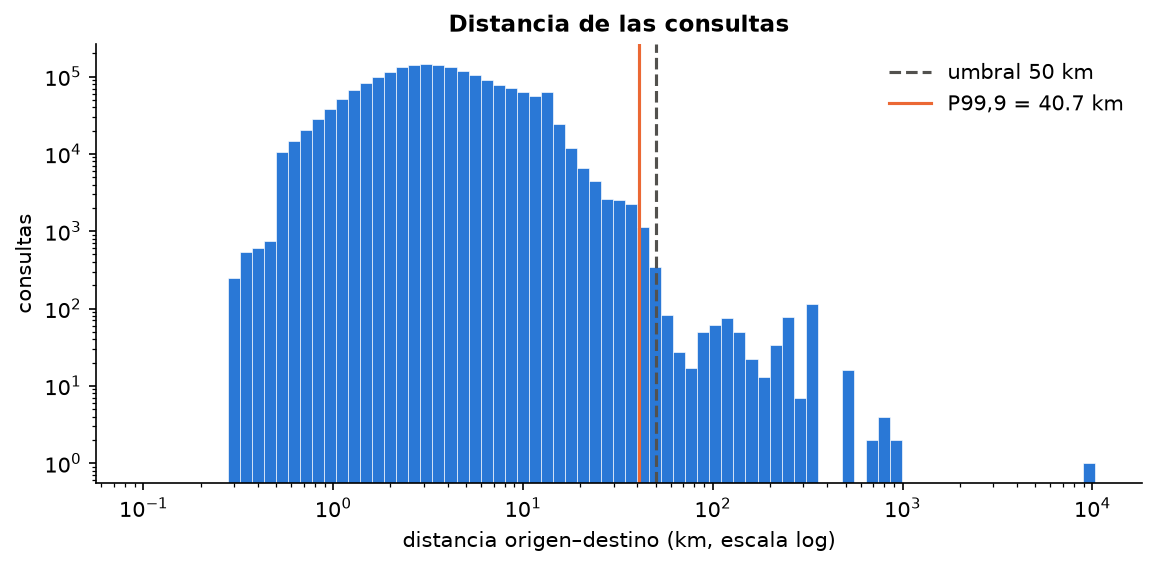
\includegraphics[width=0.75\textwidth]{imagenes/07_desarrollo/7_2_comprension_datos/distancia.png}
  \fuente{Elaboración propia, a partir de \var{01_eda} (sección 3). Ambos ejes en escala
  logarítmica; la línea discontinua marca el umbral de 50~km.}
\end{figure}

El umbral de 50~km se aplica a las \emph{consultas} y no a la delimitación del área. Una
consulta con destino lejano puede tener un origen perfectamente válido dentro de la
ciudad. Si el área se recortara con ese criterio, zonas reales quedarían fuera.

\textbf{Usuarios anómalos.} Hay 130.545 identificadores de instalación distintos. Para
detectar un uso no humano, por ejemplo pruebas automatizadas o extracción masiva de
rutas, se definieron seis señales por usuario, con umbrales fijados en \var{config.py}:
\begin{itemize}
  \item más de 1.000 consultas en total (volumen);
  \item más de 50 consultas por día activo (intensidad);
  \item más de 200 zonas de origen distintas (dispersión);
  \item más de 100 consultas en un mismo día (ráfaga);
  \item menos del 5~\% de pares origen--destino repetidos entre usuarios con más de 100
        consultas (sin rutina);
  \item un intervalo mediano menor de 60~segundos entre consultas consecutivas (rapidez).
\end{itemize}

La tabla~\ref{tab:senales-usuario} muestra cuántos usuarios activan cada señal y justifica
que se exijan al menos dos. La señal de rapidez, por sí sola, marcaría a 10.511
instalaciones. Esas instalaciones corresponden a un comportamiento humano habitual:
repetir una búsqueda o corregir el destino en pocos segundos. Exigir dos señales
simultáneas deja solo dos instalaciones anómalas, con 233 consultas en total.

\begin{table}[H]
  \centering
  \caption{Usuarios que activan cada señal de uso anómalo}
  \label{tab:senales-usuario}
  \interlineadoSimple
  \small
  \begin{tabular}{@{}lr@{}}
    \toprule
    \textbf{Señal} & \textbf{Usuarios} \\
    \midrule
    Volumen ($>$ 1.000 consultas) & 1 \\
    Intensidad ($>$ 50 consultas por día activo) & 1 \\
    Dispersión ($>$ 200 zonas de origen) & 0 \\
    Ráfaga ($>$ 100 consultas en un día) & 1 \\
    Sin rutina ($<$ 5~\% de pares repetidos) & 0 \\
    Rapidez (intervalo mediano $<$ 60~s) & 10.511 \\
    \midrule
    \textbf{Marcados como anómalos ($\geq$ 2 señales)} & \textbf{2} \\
    \bottomrule
  \end{tabular}
  \fuente{Elaboración propia, a partir de \var{resultados/01_eda/usuarios_senales.csv} y
  \var{src/limpieza.py}.}
\end{table}

\subsection{Distribución temporal y espacial}
\label{sec:distribucion-datos}

\subsubsection{Cobertura temporal}
\label{sec:cobertura-temporal}

El período declarado va del 12 de septiembre de 2022 al 9 de junio de 2024, es decir,
91 semanas ISO. Hay datos en 84 de ellas, repartidos en 85 archivos: la semana que va del
26 de diciembre de 2022 al 1 de enero de 2023 se exportó en dos archivos, uno con los días
26 a 31 de diciembre (11.622 consultas) y otro con el 1 de enero (695), sin filas repetidas
entre ambos. De las 84 semanas, 78 tienen registros los siete días. Faltan
siete semanas consecutivas, del 11 de marzo al 28 de abril de 2024, sin ninguna consulta
(figura~\ref{fig:cobertura-semanal}).

\begin{figure}[H]
  \centering
  \caption{Consultas por semana y hueco sin datos de 2024}
  \label{fig:cobertura-semanal}
  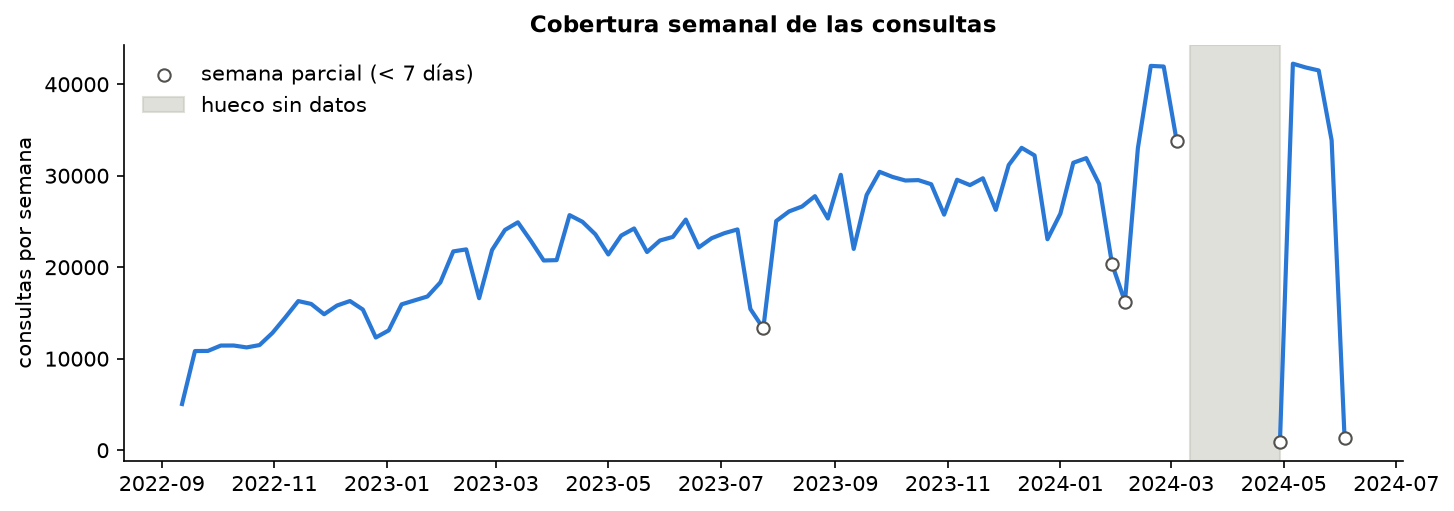
\includegraphics[width=\textwidth]{imagenes/07_desarrollo/7_2_comprension_datos/cobertura_semanal.png}
  \fuente{Elaboración propia, a partir de \var{01_eda} (sección 5). Los círculos marcan
  semanas parciales (menos de siete días con datos).}
\end{figure}

La serie muestra un crecimiento sostenido del uso: de unas 11.000 consultas semanales a
fines de 2022 a más de 30.000 a fines de 2023. La media semanal pasa de 22.731 consultas
antes del hueco a 39.864 después. El hueco coincide exactamente con el cambio de esquema:
el lote 2024, con dos columnas nuevas y otra codificación, empieza en la primera semana
posterior. Esa coincidencia sugiere una interrupción del proceso de exportación, y no una
caída real del uso.

El conjunto de datos disponible corresponde a las exportaciones que Trufi Association pudo
extraer y entregar en el plazo del proyecto; el resto del registro continúa en proceso de
exportación. El hueco de siete semanas y el cambio de esquema son consistentes con esa
interrupción, aunque la causa exacta no pudo confirmarse. Esta limitación se retoma en la
sección~\ref{sec:limitaciones} y en la recomendación R8. El registro es, por tanto,
parcial y puede ampliarse, y los resultados describen los datos entregados.

El hueco no afecta a la unidad de análisis, que es el total de consultas por zona
acumulado en todo el período. Sí afecta a la lectura de ese total como volumen semanal.
Por eso la preparación calcula las semanas equivalentes realmente observadas
(sección~\ref{sec:transformaciones}), y la evaluación comprueba si la lista de zonas
cambia al usar solo el período anterior al hueco (sección~\ref{sec:interpretacion-resultados}).

El perfil horario y semanal (figura~\ref{fig:perfil-temporal}) confirma que el registro
refleja un uso cotidiano de transporte:
\begin{itemize}
  \item la actividad crece desde las 6~h y alcanza su máximo a las 14~h, con el 8,2~\% de
        las consultas;
  \item los días laborables reúnen entre el 14~\% y el 17~\% de las consultas cada uno;
  \item el fin de semana concentra el 22,8~\%, y el domingo es el día de menor uso.
\end{itemize}
Este perfil no se modela, porque el alcance excluye la dimensión temporal. Se incluye como
evidencia de que las consultas corresponden a necesidades reales de desplazamiento y no a
tráfico artificial.

\begin{figure}[H]
  \centering
  \caption{Distribución de las consultas por hora del día y por día de la semana}
  \label{fig:perfil-temporal}
  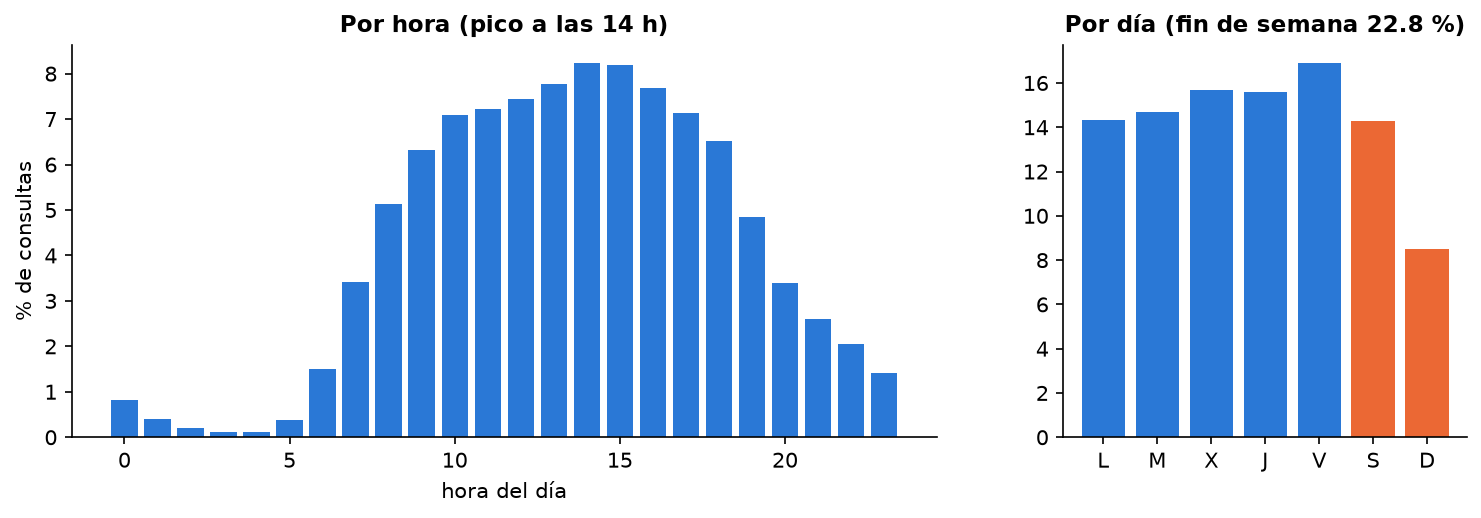
\includegraphics[width=\textwidth]{imagenes/07_desarrollo/7_2_comprension_datos/perfil_temporal.png}
  \fuente{Elaboración propia, a partir de \var{01_eda} (sección 5) y
  \var{resultados/01_eda/perfil_temporal.csv}.}
\end{figure}

\subsubsection{Distribución espacial y área de estudio}
\label{sec:area-estudio}

El alcance dejó abierta la delimitación operativa del entorno del eje metropolitano
(capítulo~\ref{cap:alcance}), y esta fase la fija a partir de los propios datos. El primer
intento fue la envolvente de todas las zonas H3 con al menos un origen válido, que
abarcaría 485.940,1~km\textsuperscript{2}, más de un tercio de la superficie de Bolivia.
El motivo es que unas pocas consultas aisladas, muy alejadas, estiran el contorno. Ese
resultado muestra que un área definida por los datos crudos es frágil ante atípicos
geográficos.

La solución adoptada identifica la \emph{componente contigua principal} de las zonas H3
con orígenes válidos. Esa componente es el mayor conjunto de zonas conectadas entre sí por
vecindad directa. El área es su envolvente, ampliada con un margen de 1~km. La
tabla~\ref{tab:variantes-area} compara esta opción con otras más laxas, en las que dos
zonas se consideran conectadas aunque estén separadas por uno o dos anillos vacíos.

\begin{table}[H]
  \centering
  \caption{Variantes de delimitación del área de estudio}
  \label{tab:variantes-area}
  \interlineadoSimple
  \small
  \begin{tabular}{@{}lrr@{}}
    \toprule
    \textbf{Variante} & \textbf{Zonas H3} & \textbf{Área (km\textsuperscript{2})} \\
    \midrule
    Todas las zonas con orígenes válidos & 1.516 & 485.940,1 \\
    \textbf{Componente contigua, vecindad directa ($k=1$)} & \textbf{919} & \textbf{1.505,7} \\
    Componente con separación de hasta un anillo ($k=2$) & 1.076 & 1.965,4 \\
    Componente con separación de hasta dos anillos ($k=3$) & 1.195 & 3.040,9 \\
    \bottomrule
  \end{tabular}
  \fuente{Elaboración propia, a partir de \var{resultados/01_eda/area_variantes.csv}. El área
  incluye el margen de 1~km.}
\end{table}

La variante elegida mide 1.505,7~km\textsuperscript{2} y contiene el 99,87~\% de los
orígenes válidos (figura~\ref{fig:area-estudio}). Las variantes más laxas duplican el área
para ganar una fracción mínima de consultas, a costa de incorporar zonas rurales casi sin
uso. Las 2.509 consultas que quedan fuera son las que la
tabla~\ref{tab:calidad-consultas} registra como ``origen fuera del área de estudio''.

\begin{figure}[H]
  \centering
  \caption{Orígenes de las consultas y área de estudio delimitada}
  \label{fig:area-estudio}
  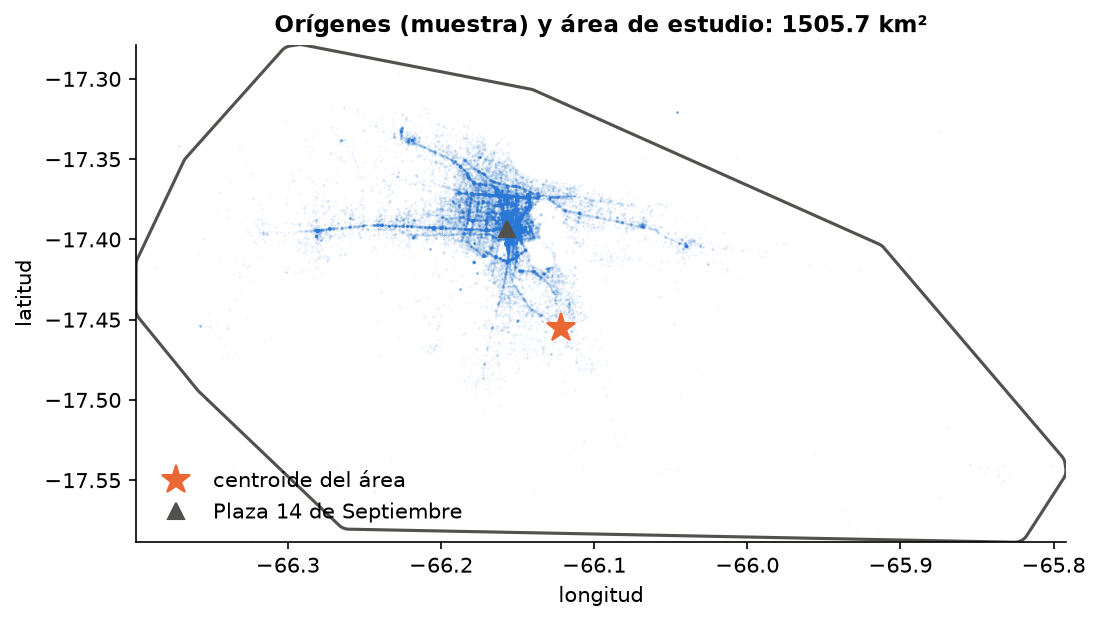
\includegraphics[width=0.85\textwidth]{imagenes/07_desarrollo/7_2_comprension_datos/area_estudio.png}
  \fuente{Elaboración propia, a partir de \var{01_eda} (sección 6). Puntos: muestra de
  orígenes; contorno: área de estudio; triángulo: Plaza 14 de Septiembre; estrella:
  centroide geométrico del área.}
\end{figure}

La figura revela además un hecho que se retoma en la preparación: el centroide geométrico
del área está a 7,82~km de la Plaza 14 de Septiembre, fuera del núcleo donde se concentran
los orígenes. Un ``centro'' calculado a partir de la forma del área no representa el
centro de actividad de la ciudad.

Dentro del área se localizan 1.577 celdas de Kontur (por la posición de su centroide), con
1.223.871 habitantes. De ellas, 609 no registran ningún origen de consulta en los datos
sin depurar; tras la limpieza son 611, porque dos celdas solo tenían consultas que la limpieza
excluyó (sección~\ref{sec:limpieza}). Además, 202 tienen
menos de 10 habitantes. La red mapeada cubre la mayor parte del territorio con demanda
(figura~\ref{fig:gtfs-red}): el 99,47~\% de los orígenes está a 500~m o menos de algún
trazado GTFS. Los trazados tienen una longitud mediana de 20,22~km y suman
12.737,3~km. La frecuencia mediana declarada es de un servicio cada 5~minutos.

\begin{figure}[H]
  \centering
  \caption{Trazados de la red mapeada (GTFS) y orígenes de las consultas}
  \label{fig:gtfs-red}
  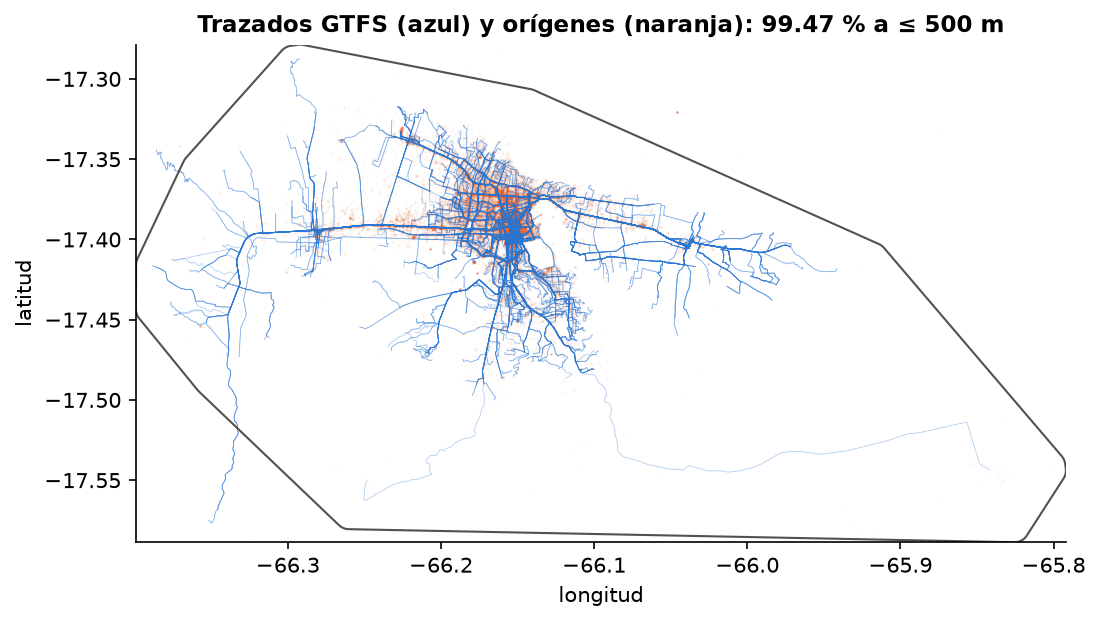
\includegraphics[width=0.85\textwidth]{imagenes/07_desarrollo/7_2_comprension_datos/gtfs_red_y_demanda.png}
  \fuente{Elaboración propia, a partir de \var{01_eda} (sección 7). Azul: trazados de
  \var{shapes.txt}; naranja: orígenes.}
\end{figure}

Que casi todos los orígenes estén cerca de un trazado no implica que la red esté completa.
Las consultas nacen donde la aplicación ya es útil: una zona sin rutas mapeadas genera
pocas consultas precisamente porque la aplicación no le ofrece respuestas. Este sesgo de
selección es la razón por la que la cobertura no puede usarse para estimar lo esperado
(sección~\ref{sec:traduccion-necesidad}). También hay que tener en cuenta que el feed
declara una vigencia posterior a buena parte del período de consultas, una limitación ya
reconocida en el capítulo~\ref{cap:alcance}.

\subsubsection{Distribución de la variable objetivo}
\label{sec:distribucion-objetivo}

La variable objetivo candidata, \var{query_count}, es el número de consultas válidas
originadas en cada zona H3 de resolución~8 durante el período. Dentro del área hay 1.628
zonas. Para que una tasa por habitante sea estable, se exige un mínimo de 10 habitantes;
1.381 zonas lo cumplen. La figura~\ref{fig:objetivo-distribucion} resume la distribución
del conteo en esas 1.381 zonas.

\begin{figure}[H]
  \centering
  \caption{Distribución del conteo de consultas por zona y curva de Lorenz}
  \label{fig:objetivo-distribucion}
  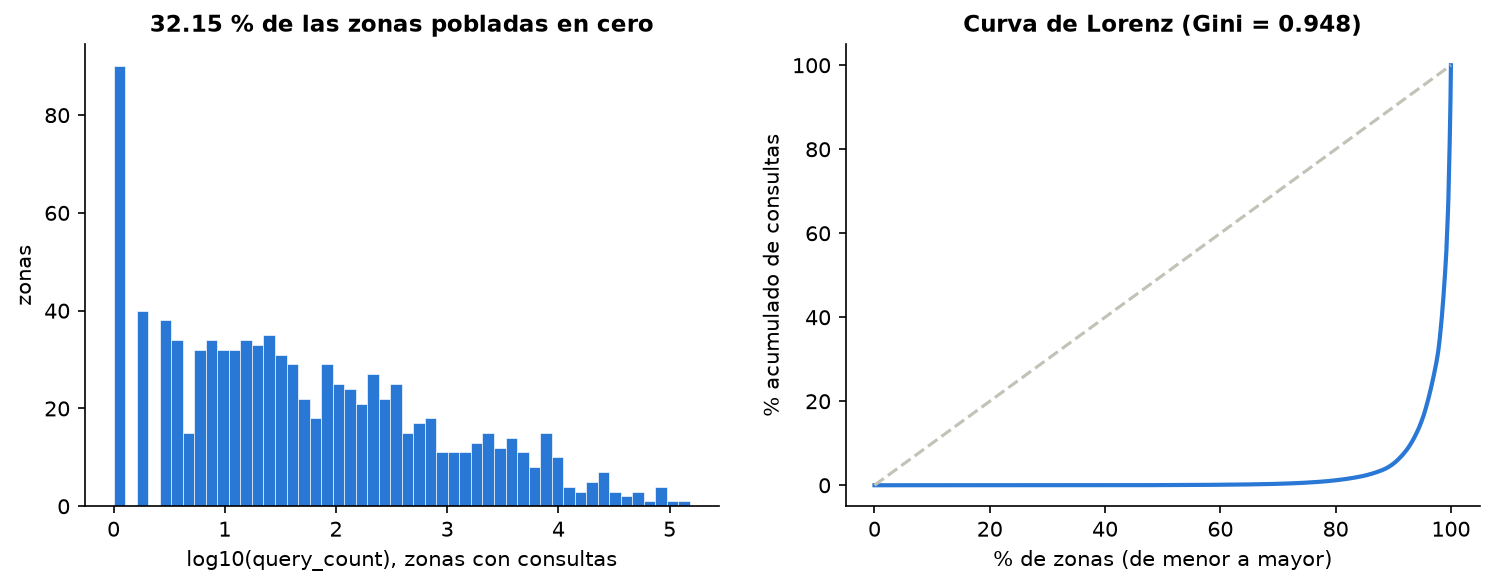
\includegraphics[width=\textwidth]{imagenes/07_desarrollo/7_2_comprension_datos/objetivo_distribucion.png}
  \fuente{Elaboración propia, a partir de \var{01_eda} (sección 9). Izquierda: histograma de
  $\log_{10}$ del conteo en las zonas con consultas; derecha: proporción acumulada de
  consultas frente a proporción acumulada de zonas.}
\end{figure}

Tres rasgos caracterizan la distribución y condicionan el modelado:
\begin{itemize}
  \item \textbf{Abundancia de ceros.} El 32,15~\% de las zonas pobladas (444 de 1.381) no
        registra ninguna consulta. Esos ceros se conservan: son justamente el tipo de zona
        que el problema busca examinar (capítulo~\ref{cap:problema}).
  \item \textbf{Concentración extrema.} El coeficiente de Gini es de 0,948, y las diez
        zonas con más consultas reúnen el 42~\% del total. Como muestra la curva de Lorenz,
        el 80~\% de las zonas aporta menos del 5~\% de las consultas.
  \item \textbf{Sobredispersión.} La varianza del conteo es 46.569 veces su media. Un modelo
        de Poisson supone varianza igual a la media
        (sección~\ref{subsec:datos-conteo}), así que este resultado anticipa que ese
        supuesto no se cumplirá y justifica incluir alternativas que lo relajen.
\end{itemize}

\subsection{Relaciones entre variables y dependencia espacial}
\label{sec:relaciones-variables}

Para examinar qué información territorial se asocia con las consultas, se calculó la
correlación de Spearman entre el conteo por zona y cada variable candidata. La correlación
de Spearman se basa en rangos, por lo que es robusta a la asimetría de los datos. Se
calculó también frente a la \emph{tasa} de consultas por 1.000 habitantes, para distinguir
la asociación que se debe solo al tamaño de la población de la que se debe al contexto. La
tabla~\ref{tab:relaciones} presenta los resultados.

\begin{table}[H]
  \centering
  \caption{Correlación de Spearman de las variables candidatas con el conteo y con la tasa}
  \label{tab:relaciones}
  \interlineadoSimple
  \small
  \begin{tabularx}{\textwidth}{@{}L{0.22\textwidth}Yrr@{}}
    \toprule
    \textbf{Variable} & \textbf{Significado} & \textbf{Conteo} & \textbf{Tasa} \\
    \midrule
    \var{population} & Habitantes de la zona (Kontur) & 0,855 & 0,710 \\
    \var{pop_ring1} & Habitantes del primer anillo de seis zonas vecinas & 0,836 & 0,721 \\
    \var{pop_ring2} & Habitantes del segundo anillo de vecinas & 0,804 & 0,701 \\
    \var{dist_centro_km} & Distancia a la Plaza 14 de Septiembre (km) & $-0{,}697$ & $-0{,}677$ \\
    \var{dist_centroide_km} & Distancia al centroide geométrico del área (km) & $-0{,}476$ & $-0{,}485$ \\
    \var{dist_trazado_m} & Distancia al trazado GTFS más cercano (m); solo contraste & $-0{,}763$ & $-0{,}701$ \\
    \bottomrule
  \end{tabularx}
  \fuente{Elaboración propia, a partir de \var{resultados/01_eda/relaciones.csv}; 1.381 zonas
  con al menos 10 habitantes.}
\end{table}

De la tabla se desprenden tres lecturas:
\begin{itemize}
  \item La población es la variable más asociada con el conteo, lo que justifica tratarla
        como exposición. Las variables de entorno siguen asociadas con la \emph{tasa}
        (0,72 para la población vecina y $-0{,}68$ para la distancia al centro), de modo que
        el contexto aporta información más allá del tamaño de la zona.
  \item La distancia a la Plaza se asocia bastante más que la distancia al centroide del
        área ($-0{,}697$ frente a $-0{,}476$), lo que confirma que el centro de referencia
        debe fijarse de forma externa a los datos y no derivarse de la forma del área.
  \item La distancia al trazado GTFS tiene una asociación fuerte, pero se reserva para el
        contraste por el sesgo de selección descrito en la sección~\ref{sec:area-estudio}.
\end{itemize}

La figura~\ref{fig:objetivo-poblacion} muestra la relación con la población en escala
logarítmica. La asociación es clara, pero la dispersión es enorme: zonas con población
similar difieren en varios órdenes de magnitud. Las zonas alejadas del trazado (en
naranja) se concentran en la parte baja.

\begin{figure}[H]
  \centering
  \caption{Consultas por zona frente a su población, según la distancia al trazado}
  \label{fig:objetivo-poblacion}
  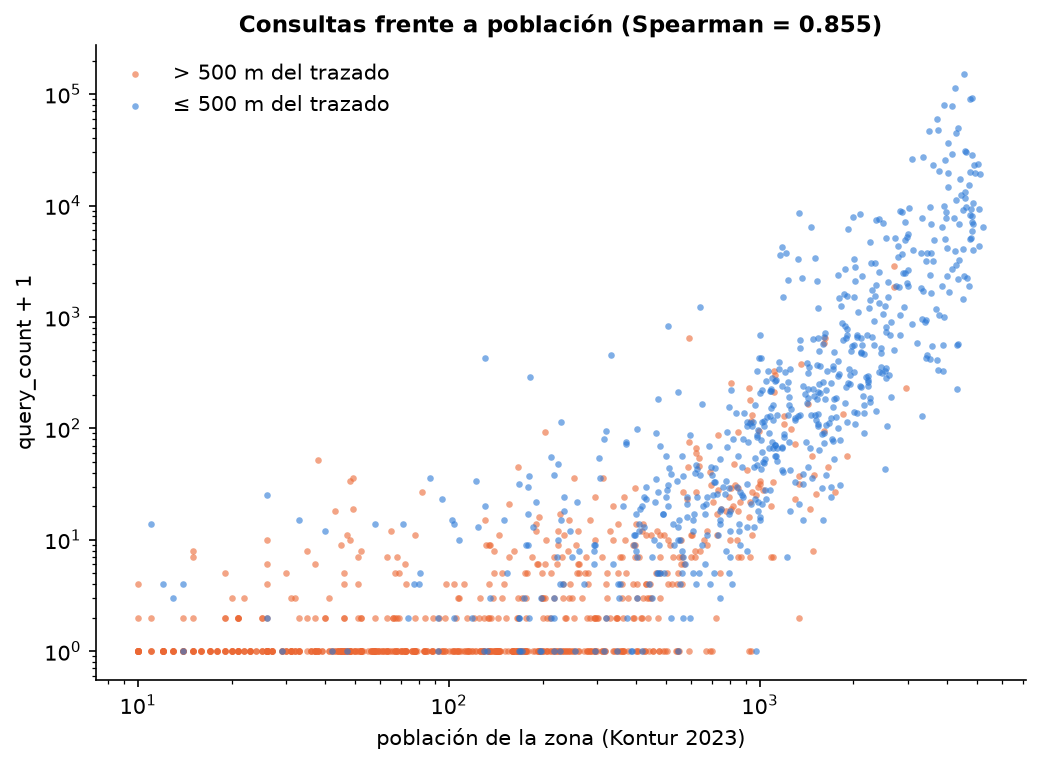
\includegraphics[width=0.75\textwidth]{imagenes/07_desarrollo/7_2_comprension_datos/objetivo_vs_poblacion.png}
  \fuente{Elaboración propia, a partir de \var{01_eda} (sección 10). Ambos ejes en escala
  logarítmica; al conteo se le suma 1 para representar los ceros.}
\end{figure}

\textbf{Dependencia espacial.} Se midió con el índice $I$ de Moran de la tasa de consultas
(sección~\ref{subsec:autocorrelacion}), tomando como vecinas las zonas situadas a $k$
anillos H3 de distancia, con $k$ de 1 a 5. La significación se evaluó con 499
permutaciones, por lo que el menor $p$-valor alcanzable es 0,002.

\begin{table}[H]
  \centering
  \caption{Correlograma del índice de Moran de la tasa de consultas}
  \label{tab:correlograma}
  \interlineadoSimple
  \small
  \begin{tabular}{@{}crrr@{}}
    \toprule
    \textbf{\celda{Orden de\\vecindad $k$}} & \textbf{\celda{Distancia\\aproximada (km)}} & \textbf{$I$ de Moran} & \textbf{$p$-valor} \\
    \midrule
    1 & 0,92 & 0,7161 & 0,002 \\
    2 & 1,84 & 0,6399 & 0,002 \\
    3 & 2,76 & 0,5773 & 0,002 \\
    4 & 3,68 & 0,5094 & 0,002 \\
    5 & 4,60 & 0,4603 & 0,002 \\
    \bottomrule
  \end{tabular}
  \fuente{Elaboración propia, a partir de \var{resultados/01_eda/autocorrelacion.csv}.}
\end{table}

El correlograma (tabla~\ref{tab:correlograma}) muestra una autocorrelación positiva muy
fuerte entre vecinas inmediatas ($I = 0{,}72$), que decae lentamente y sigue en 0,46 a
unos 4,6~km. El indicador local LISA (figura~\ref{fig:lisa}) localiza esa estructura:
\begin{itemize}
  \item un gran núcleo de 295 zonas \emph{alto-alto} (tasa alta rodeada de tasas altas) en
        el centro y los ejes de Cercado y Sacaba;
  \item 253 zonas \emph{bajo-bajo} en la periferia y en el sur del valle;
  \item pocos casos discordantes (41 alto-bajo y 3 bajo-alto).
\end{itemize}

\begin{figure}[H]
  \centering
  \caption{Agrupamientos locales de la tasa de consultas (LISA)}
  \label{fig:lisa}
  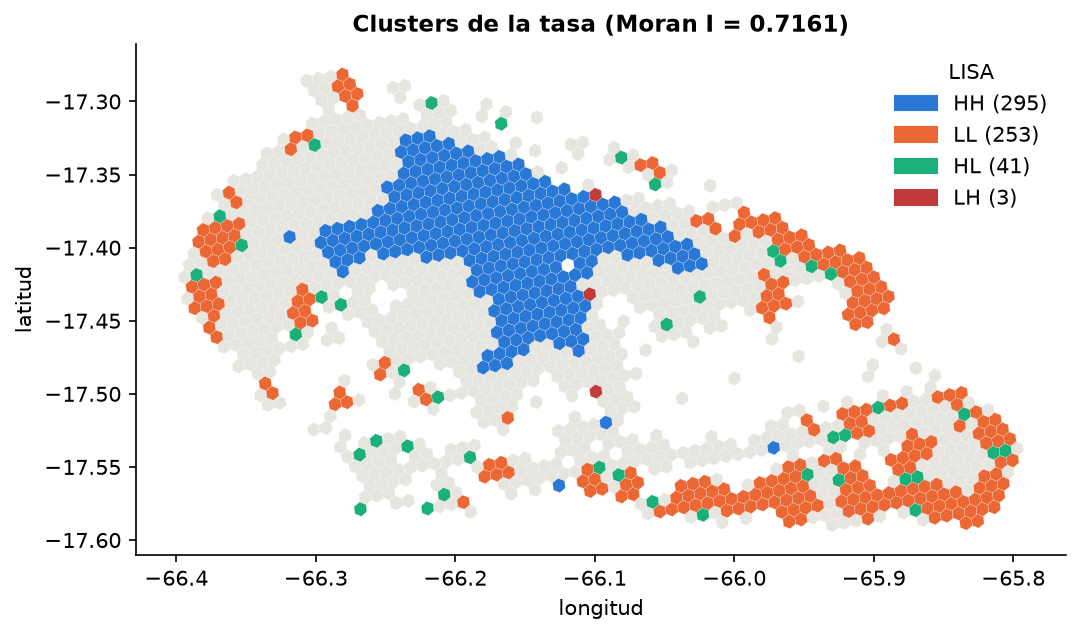
\includegraphics[width=0.85\textwidth]{imagenes/07_desarrollo/7_2_comprension_datos/lisa.png}
  \fuente{Elaboración propia, a partir de \var{01_eda} (sección 11). HH: alto-alto;
  LL: bajo-bajo; HL: alto-bajo; LH: bajo-alto; gris: sin agrupamiento significativo.}
\end{figure}

Este hallazgo tiene dos consecuencias metodológicas directas:
\begin{itemize}
  \item Las zonas vecinas se parecen, de modo que una partición aleatoria en entrenamiento
        y prueba colocaría a cada zona de prueba junto a vecinas casi idénticas y
        sobreestimaría el desempeño. La validación y la reserva de prueba deben hacerse por
        \emph{bloques} espaciales de varios kilómetros (sección~\ref{subsec:validacion-espacial}).
  \item La tasa de las zonas vecinas contiene información útil para estimar la de una zona,
        lo que motiva incluir entre las técnicas un estimador de vecindad
        (sección~\ref{sec:seleccion-algoritmos}).
\end{itemize}

\subsection{Estadísticas descriptivas del conjunto de datos H3}
\label{sec:estadisticas-descriptivas}

La tabla~\ref{tab:descriptivos} reúne las estadísticas de las variables numéricas por zona
que se usan en las fases siguientes. Se calculan sobre las 1.381 zonas que entrarán al
modelo.

\begin{table}[H]
  \centering
  \caption{Estadísticas descriptivas de las variables por zona}
  \label{tab:descriptivos}
  \interlineadoSimple
  \small
  \begin{tabular}{@{}lrrrrrrr@{}}
    \toprule
    \textbf{Variable} & \textbf{Media} & \textbf{Desv. est.} & \textbf{Mín.} & \textbf{P25} & \textbf{Mediana} & \textbf{P75} & \textbf{Máx.} \\
    \midrule
    \var{query_count} (consultas) & 1.393,4 & 8.058,4 & 0 & 0 & 6 & 109 & 152.494 \\
    \var{population} (hab.) & 887,5 & 1.162,6 & 10 & 97 & 388 & 1.183 & 5.240 \\
    \var{pop_ring1} (hab.) & 5.221,8 & 6.363,6 & 3 & 799 & 2.398 & 7.613 & 28.988 \\
    \var{dist_centro_km} (km) & 17,0 & 9,4 & 0,5 & 9,7 & 15,9 & 22,1 & 41,8 \\
    \bottomrule
  \end{tabular}
  \fuente{Elaboración propia, a partir de
  \var{resultados/03_feature_engineering/estadisticas_descriptivas.csv}; 1.381 zonas con al
  menos 10 habitantes.}
\end{table}

La distancia entre la media (1.393 consultas) y la mediana (6) del conteo resume la
asimetría: la zona típica tiene muy pocas consultas, y un puñado de zonas centrales
concentra casi todo el volumen. El percentil 25 del conteo es 0, reflejo del 32~\% de
zonas pobladas sin consultas. En cuanto a la cobertura, algo más de la mitad de las zonas
del modelo no tiene un trazado a 500~m o menos: son 755 zonas (el 54,7~\%), pero reúnen
solo 200.041 habitantes, el 16~\% de la población del modelo
(\var{resultados/05_evaluacion/contraste_gtfs.csv}).

Las tablas~\ref{tab:descriptivos}, \ref{tab:municipios} y~\ref{tab:anillos} se calculan en
\var{03_feature_engineering} y se guardan en
\var{resultados/03_feature_engineering/estadisticas_descriptivas.csv},
\var{resumen_municipio.csv} y \var{resumen_anillo.csv}, respectivamente.

\subsection{Registro de hallazgos y decisiones}
\label{sec:hallazgos-decisiones}

La tabla~\ref{tab:trazabilidad-hallazgos} reúne los hallazgos de esta fase que modifican
alguna decisión posterior. Cada uno se vincula con la fase en la que actúa. Los hallazgos
descriptivos que no cambian ninguna decisión, como el perfil horario, no se incluyen.

\begin{table}[H]
  \centering
  \caption{Hallazgos de la comprensión de los datos y decisiones que habilitan}
  \label{tab:trazabilidad-hallazgos}
  \interlineadoSimple
  \small
  \begin{tabularx}{\textwidth}{@{}L{0.30\textwidth}YL{0.16\textwidth}@{}}
    \toprule
    \textbf{Hallazgo} & \textbf{Decisión} & \textbf{Fase} \\
    \midrule
    La envolvente de todos los orígenes abarca 485.940~km\textsuperscript{2} & Área = componente H3 contigua más 1~km (1.505,7~km\textsuperscript{2}) & Preparación \\
    Cola de distancias mayores de 50~km (0,04~\%) & Excluir esas consultas, sin recortar el área & Preparación \\
    Una sola señal marca a 10.511 usuarios legítimos & Usuario anómalo = al menos 2 de 6 señales (2 usuarios) & Preparación \\
    60 copias exactas & Conservar la primera aparición & Preparación \\
    Hueco de 7 semanas en 2024 & No imputar; expresar lo esperado por semana observada; sensibilidad sin el período posterior & Preparación y evaluación \\
    32,15~\% de zonas pobladas sin consultas & Conservar los ceros; no imputar & Preparación y modelado \\
    El centroide del área no representa el centro de actividad & Centro de referencia exógeno: Plaza 14 de Septiembre & Preparación \\
    Autocorrelación espacial persistente hasta unos 4,6~km & Validación y prueba por bloques H3 de resolución~6 (unos 36~km\textsuperscript{2}); estimador de vecindad entre las técnicas & Preparación y modelado \\
    Varianza 46.569 veces la media & Modelos de conteo con la población como exposición; incluir la binomial negativa & Modelado \\
    Orígenes concentrados cerca de la red mapeada & GTFS solo para contraste, nunca como predictor & Preparación y evaluación \\
    \bottomrule
  \end{tabularx}
  \fuente{Elaboración propia, a partir de \var{01_eda} (sección 13, cierre).}
\end{table}

Todos los hallazgos se relacionan con el objetivo general. Los que afectan al área, a los
ceros y a la exposición determinan el universo de zonas sobre el que se estima lo
esperado. Los que afectan a la dependencia espacial determinan cómo se medirá la
confiabilidad de esa estimación en zonas no observadas. El que afecta a la red mapeada
preserva la posibilidad de contrastar la brecha con la cobertura sin que el modelo la
absorba.

% ============================================================
%  7.3. PREPARACIÓN DE LOS DATOS  -- parte del capítulo 7
%  ------------------------------------------------------------
%  Guía 2.7.3: (1) datos seleccionados y por qué, (2) limpieza,
%  faltantes y atípicos, (3) transformaciones y codificación,
%  (4) ingeniería y selección de características, (5) conjuntos
%  de entrenamiento y prueba. Justificar, no enumerar comandos.
%  Notebooks: 02_preprocesamiento.ipynb (limpieza, data/interim/)
%             03_feature_engineering.ipynb (variables, partición,
%             data/processed/tabla_modelado.parquet)
% ============================================================
\section{Preparación de los datos}
\label{sec:preparacion-datos}

La preparación convierte las fuentes crudas en el conjunto de datos H3 sobre el que se modela.
Aplica, en el orden fijado por la sección~\ref{sec:hallazgos-decisiones}, los criterios que
el análisis exploratorio solo había medido. Se ejecuta en dos notebooks:
\begin{itemize}
  \item \var{02_preprocesamiento} limpia las consultas y construye el conjunto de datos H3 por zona, que
        guarda en \var{data/interim/}.
  \item \var{03_feature_engineering} añade las variables, declara cuáles serán predictores y
        reserva el conjunto de prueba. Su resultado es
        \var{data/processed/tabla_modelado.parquet}, con 1.628 filas y 18 columnas.
\end{itemize}
Todos los umbrales viven en un único archivo de configuración (\var{config.py}), de modo
que ninguna cifra se escribe a mano dentro de los notebooks.

\subsection{Selección de los datos}
\label{sec:seleccion-datos}

Se seleccionan tres conjuntos, cada uno por una razón distinta.

\textbf{Consultas.} Se conservan todas las consultas válidas del período completo, sin
muestreo. El problema se formula sobre el total acumulado por zona
(capítulo~\ref{cap:problema}), y descartar semanas o usuarios reduciría la información de
las zonas con poca actividad, que son precisamente las de interés.

\textbf{Zonas.} El conjunto de datos H3 se construye como la unión de dos conjuntos: las celdas
de Kontur cuyo centroide cae dentro del área de estudio (1.577) y las celdas donde se
originó al menos una consulta válida. Esta unión es deliberada. Si solo se tomaran las
zonas con consultas, desaparecerían las 611 zonas pobladas sin ninguna consulta, que son
el tipo de zona que el proyecto debe poder señalar. Si solo se tomaran las celdas de
Kontur, se perderían 51 zonas con consultas situadas en el borde del área. El resultado
son 1.628 zonas: 1.017 con consultas y 611 pobladas sin consultas
(figura~\ref{fig:consultas-por-zona}).

\begin{figure}[H]
  \centering
  \caption{Consultas por zona y zonas pobladas sin consultas}
  \label{fig:consultas-por-zona}
  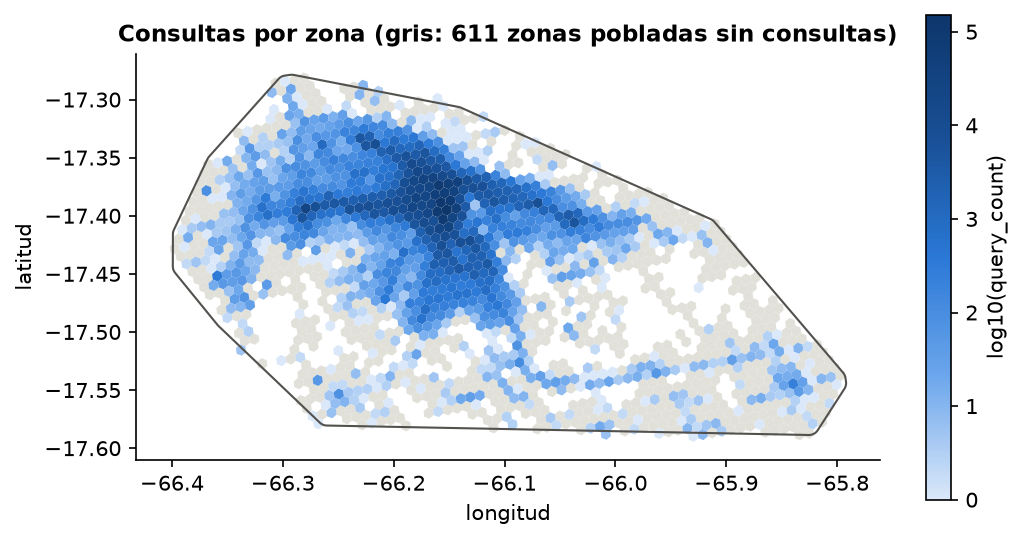
\includegraphics[width=0.85\textwidth]{imagenes/07_desarrollo/7_3_preparacion/consultas_por_zona.png}
  \fuente{Elaboración propia, a partir de \var{02_preprocesamiento} (sección 8). Escala de
  color: $\log_{10}$ del conteo; gris: zonas pobladas sin consultas.}
\end{figure}

Las zonas sin consultas no se distribuyen al azar: se concentran en la periferia del
valle y en el sur del área, lejos del núcleo donde el color es más intenso. Si se
eliminaran, la tabla describiría solo el territorio donde la aplicación ya se usa.

\textbf{Zonas del modelo.} De las 1.628 zonas, entran al modelo las que tienen al menos
10 habitantes, que son 1.381. La tabla~\ref{tab:zonas-modelo} muestra qué se excluye. El
motivo es técnico: el modelo estima una tasa por habitante, y con muy pocos habitantes esa
tasa se vuelve inestable (una sola consulta en una zona de 2 habitantes equivale a 500 por
cada 1.000). Las zonas sin población no pueden entrar, porque la exposición sería cero. La
exclusión apenas afecta al volumen: se pierden 242 consultas, y el modelo conserva
1.924.336 de las 1.924.578 consultas válidas (el 99,99~\%).

\begin{table}[H]
  \centering
  \caption{Zonas del área de estudio según su población}
  \label{tab:zonas-modelo}
  \interlineadoSimple
  \small
  \begin{tabular}{@{}lrr@{}}
    \toprule
    \textbf{Grupo} & \textbf{Zonas} & \textbf{Consultas} \\
    \midrule
    Sin población en Kontur (\var{population} $= 0$) & 43 & 102 \\
    Entre 1 y 9 habitantes & 204 & 140 \\
    \textbf{Al menos 10 habitantes (zonas del modelo)} & \textbf{1.381} & \textbf{1.924.336} \\
    \midrule
    Total & 1.628 & 1.924.578 \\
    \bottomrule
  \end{tabular}
  \fuente{Elaboración propia, a partir de
  \var{resultados/03_feature_engineering/zonas_por_grupo.csv}.}
\end{table}

La población total de las 1.628 zonas es de 1.226.308 habitantes, algo más que los
1.223.871 de las celdas de Kontur situadas dentro del área
(sección~\ref{sec:area-estudio}). La diferencia, de 2.437 habitantes, proviene de las
zonas de borde incorporadas por tener consultas: su centroide queda fuera del contorno,
pero Kontur les asigna población.

\subsection{Limpieza, datos faltantes y valores atípicos}
\label{sec:limpieza}

\textbf{Consolidación.} Los 85 archivos, que cubren 84 semanas con datos (una semana viene
partida en dos archivos; sección~\ref{sec:cobertura-temporal}), se leen con detección automática de codificación:
se intenta UTF-8 y, si falla, Latin-1. Así se leen correctamente los seis archivos del
lote 2024 y los nombres con tildes (por ejemplo, ``Santivañez''). Las columnas
equivalentes de ambos esquemas se unifican, y a cada fila se le añade su linaje. Las
consultas se ordenan de forma estable (archivo, marca de tiempo, usuario y coordenadas),
para que cualquier ejecución produzca exactamente el mismo resultado.

\textbf{Filtros.} Se aplican seis filtros en un orden fijo, que va de lo inequívoco a lo
que depende de decisiones. La tabla~\ref{tab:flujo-filtros} y la
figura~\ref{fig:flujo-limpieza} muestran cuántas consultas elimina cada paso.

\begin{table}[H]
  \centering
  \caption{Flujo de limpieza de las consultas}
  \label{tab:flujo-filtros}
  \interlineadoSimple
  \small
  \begin{tabularx}{\textwidth}{@{}clrrY@{}}
    \toprule
    \textbf{Paso} & \textbf{Regla} & \textbf{Eliminadas} & \textbf{Quedan} & \textbf{Justificación} \\
    \midrule
    0 & Consultas crudas & --- & 1.927.675 & --- \\
    1 & Origen en (0,0) & 3 & 1.927.672 & Coordenadas no localizables \\
    2 & Origen fuera de Bolivia & 9 & 1.927.663 & Coordenadas imposibles para el servicio \\
    3 & Copia de duplicado exacto & 60 & 1.927.603 & Se conserva la primera aparición \\
    4 & Origen fuera del área & 2.509 & 1.925.094 & Área fijada en la sección~\ref{sec:area-estudio} \\
    5 & Distancia $>$ 50~km & 283 & 1.924.811 & Fuera de la escala urbana (sección~\ref{sec:atipicos}) \\
    6 & Usuario anómalo & 233 & 1.924.578 & Al menos 2 de 6 señales (sección~\ref{sec:atipicos}) \\
    \bottomrule
  \end{tabularx}
  \fuente{Elaboración propia, a partir de
  \var{resultados/02_preprocesamiento/flujo_limpieza.csv}. Se conserva el 99,84~\% de las
  consultas.}
\end{table}

\begin{figure}[H]
  \centering
  \caption{Consultas eliminadas en cada paso de la limpieza}
  \label{fig:flujo-limpieza}
  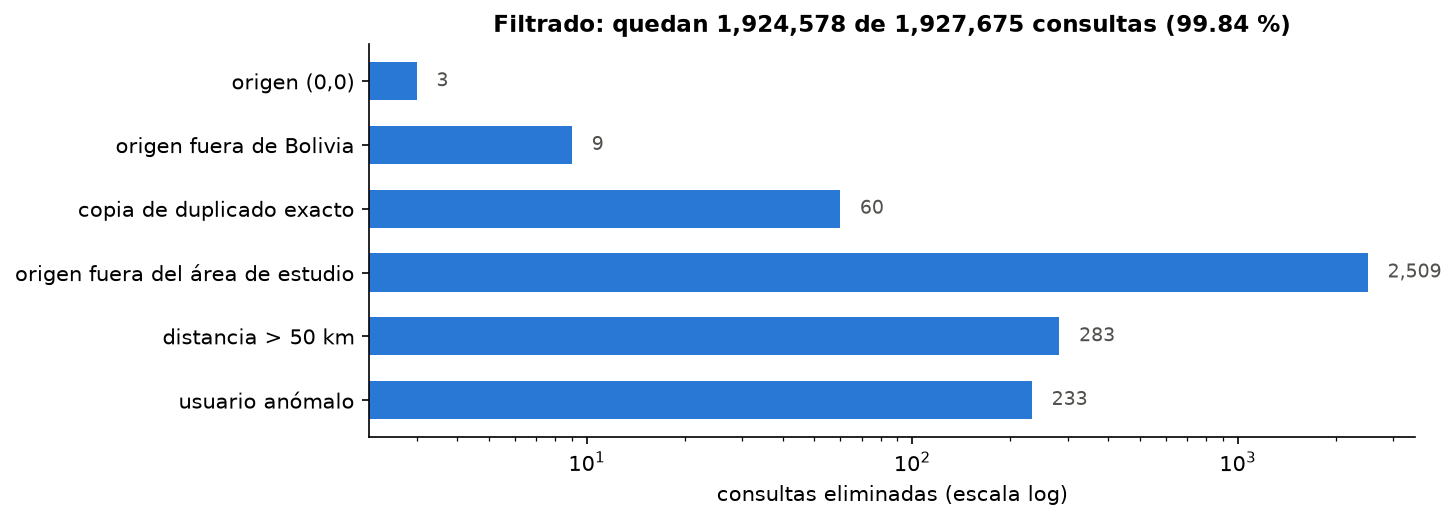
\includegraphics[width=0.9\textwidth]{imagenes/07_desarrollo/7_3_preparacion/flujo_limpieza.png}
  \fuente{Elaboración propia, a partir de \var{02_preprocesamiento} (sección 5). Eje
  horizontal en escala logarítmica.}
\end{figure}

El orden importa por dos motivos. Primero, los filtros geográficos inequívocos (pasos 1 y
2) van antes que la detección de duplicados, para que las coordenadas imposibles no
cuenten como consultas válidas. Segundo, el área de estudio (paso 4) se delimitó con los
orígenes de usuarios no anómalos y \emph{sin} aplicar el umbral de distancia, de modo que
los dos criterios no se contaminan entre sí. La mayor exclusión, la de consultas fuera del
área, representa apenas el 0,13~\% del total. En conjunto, la limpieza no altera la
estructura de los datos: corrige errores puntuales. Las cifras coinciden exactamente con
las que midió el análisis exploratorio, porque ambos notebooks usan las mismas funciones.

\textbf{Datos faltantes.} La limpieza no imputa ningún valor, por tres razones:
\begin{itemize}
  \item Las columnas que usa el proyecto no tienen nulos
        (sección~\ref{sec:datos-faltantes-eda}).
  \item Las 611 zonas pobladas sin consultas reciben un conteo de 0, que es su valor
        observado. No se trata como faltante.
  \item Las 43 zonas con consultas pero sin registro en Kontur reciben población 0. Es una
        ausencia estructural de la fuente, no un dato que deba estimarse; esas zonas quedan
        fuera del modelo por el umbral de población.
\end{itemize}
Las siete semanas sin datos tampoco se rellenan. Se registran para calcular las semanas
realmente observadas (sección~\ref{sec:transformaciones}).

\textbf{Valores atípicos.} Solo se eliminan los atípicos que representan errores o un uso
no humano: la distancia de más de 50~km y los usuarios anómalos. Los valores extremos
legítimos se conservan. Por ejemplo, la zona con más consultas acumula 152.494, frente a
una mediana de 6. Esas zonas son reales, están en el centro de la ciudad y forman parte
del fenómeno. Su efecto se controla con métricas y modelos propios de datos de conteo, no
eliminándolas.

\subsection{Transformaciones y codificación de variables}
\label{sec:transformaciones}

Las transformaciones convierten consultas individuales en un conjunto de datos H3 por zona y dejan cada
variable en la escala que requieren los modelos. La tabla~\ref{tab:transformaciones} las
resume con su justificación.

\begin{table}[H]
  \centering
  \caption{Transformaciones y codificación aplicadas}
  \label{tab:transformaciones}
  \interlineadoSimple
  \small
  \begin{tabularx}{\textwidth}{@{}L{0.26\textwidth}L{0.34\textwidth}Y@{}}
    \toprule
    \textbf{Transformación} & \textbf{Qué hace} & \textbf{Por qué} \\
    \midrule
    Asignación de zona & Convierte las coordenadas de origen en su celda H3 de resolución~8 (\var{h3_origin}) & Unidad de análisis común con Kontur, sin reproyección (sección~\ref{subsec:h3}) \\
    Agregación & Cuenta las consultas por zona de origen (\var{query_count}) & La variable objetivo es el total del período \\
    Bloque espacial & Asigna a cada zona su celda madre H3 de resolución~6 (\var{block_id}), de unos 36~km\textsuperscript{2} & Unidad de validación y de reserva de prueba \\
    Semanas equivalentes observadas & $W_{obs} = \text{días con datos} / 7 = 568/7 = 81{,}143$ & Expresar lo esperado por semana sin contar el hueco \\
    Exposición & $\log(\text{population})$ como \emph{offset} (coeficiente fijo igual a 1) & Modelar la tasa por habitante (sección~\ref{subsec:glm-poisson}) \\
    Escala de población & $\log(1 + x)$ en \var{pop_ring1} dentro de los modelos & Reduce la asimetría; no depende de los datos, así que no filtra información \\
    Municipio & Municipio más frecuente entre los orígenes de la zona; sin consultas, el de las zonas vecinas etiquetadas más cercanas & Estrato de la línea base B1 \\
    Anillo de distancia & Cuatro anillos (A1 a A4) según los cuartiles de la distancia media de cada bloque a la Plaza & Estrato de la línea base B2 y del sorteo de prueba \\
    \bottomrule
  \end{tabularx}
  \fuente{Elaboración propia, a partir de \var{src/features.py}, \var{src/modelos.py},
  \var{src/limpieza.py} y \var{resultados/02_preprocesamiento/metricas.json}.}
\end{table}

\textbf{Semanas equivalentes observadas ($W_{obs}$).} Hubo datos 538 días antes del hueco
y 30 después, 568 días en total, que equivalen a 81,143 semanas. Todos los modelos estiman
el total del período. Para comunicar el resultado a la organización en una unidad
intuitiva (consultas por semana), ese total se divide por $W_{obs}$ y no por las 91
semanas calendario. Dividir por 91 subestimaría el ritmo semanal, porque contaría semanas
en las que no se registró nada.

\textbf{Codificación de las variables categóricas.} El municipio y el anillo no se
convierten en variables indicadoras (\emph{one-hot}), porque ningún modelo los usa como
predictores. Sirven para definir los estratos de dos líneas base, que calculan una tasa
separada por grupo.

La etiqueta de municipio proviene del campo \var{origin_municipio} de las exportaciones de
Trufi Association, no de límites oficiales, y queda asignada a 14 municipios
(tabla~\ref{tab:municipios}). El municipio figura como ``Cochabamba'' en los datos, pero
corresponde a Cercado. Para comprobar si esa etiqueta es coherente dentro de cada zona, se
verificó su pureza. El 99,38~\% de las consultas comparte la etiqueta modal de su zona. Solo
el 5,02~\% de las zonas con consultas es de municipio \emph{mixto}, es decir, tiene menos
del 90~\% de sus consultas con la etiqueta modal. El único caso llamativo, Arani (50~\%),
corresponde a una zona con apenas dos consultas.

Esta decisión es aceptable para el propósito del proyecto porque el municipio se usa
únicamente como estrato en la línea base B1, que no fue la técnica seleccionada; ningún
modelo que participa en la selección final lo usa como predictor. Los resultados se
guardan en \var{resultados/03_feature_engineering/resumen_municipio.csv} y en
\var{metricas.json} (\var{pct_consultas_municipio_modal},
\var{pct_zonas_municipio_mixto}).

\begin{table}[H]
  \centering
  \caption{Zonas del modelo por municipio asignado y pureza de la etiqueta}
  \label{tab:municipios}
  \interlineadoSimple
  \small
  \begin{tabular}{@{}lrrrrr@{}}
    \toprule
    \textbf{Municipio} & \textbf{Zonas} & \textbf{Consultas} & \textbf{Población} & \textbf{\celda{\% consultas con\\etiqueta modal}} & \textbf{\celda{Zonas\\mixtas}} \\
    \midrule
    Cochabamba (Cercado) & 318 & 1.662.310 & 622.120 & 99,69 & 13 \\
    Sacaba & 259 & 90.113 & 180.427 & 99,99 & 1 \\
    Quillacollo & 137 & 65.275 & 146.291 & 97,71 & 12 \\
    Colcapirhua & 35 & 53.209 & 47.652 & 97,17 & 5 \\
    Tiquipaya & 47 & 46.785 & 60.991 & 92,27 & 7 \\
    Vinto & 89 & 3.403 & 56.167 & 95,53 & 4 \\
    Sipe Sipe & 92 & 1.357 & 35.950 & 99,78 & 2 \\
    Arbieto & 86 & 546 & 17.368 & 97,99 & 1 \\
    Villa Punata & 74 & 488 & 23.430 & 100,00 & 0 \\
    Tolata & 37 & 302 & 5.115 & 100,00 & 0 \\
    Villa Santivañez & 79 & 300 & 4.163 & 100,00 & 0 \\
    Villa José Quintín Mendoza & 76 & 170 & 13.386 & 99,41 & 1 \\
    Cliza & 47 & 76 & 11.604 & 100,00 & 0 \\
    Arani & 5 & 2 & 1.015 & 50,00 & 1 \\
    \midrule
    Total & 1.381 & 1.924.336 & 1.225.679 & 99,38 & 47 \\
    \bottomrule
  \end{tabular}
  \fuente{Elaboración propia, a partir de
  \var{resultados/03_feature_engineering/resumen_municipio.csv} y \var{metricas.json}. Zona
  mixta: menos del 90~\% de sus consultas con la etiqueta modal.}
\end{table}

La tabla muestra por qué el área de estudio excede los siete municipios del eje
metropolitano mencionados en el alcance. La componente contigua de orígenes se extiende
hacia el valle alto y el sur (Arbieto, Santivañez, Punata, Cliza, Tolata). Esos
municipios aportan muchas zonas pobladas, pero casi ninguna consulta. Cercado concentra el
86~\% de las consultas con el 51~\% de la población.

\subsection{Ingeniería y selección de características}
\label{sec:ingenieria-caracteristicas}

Cada columna del conjunto de datos H3 tiene un papel declarado antes de modelar. La
tabla~\ref{tab:grupos-variables} organiza las variables por su uso. Distinguir estos
papeles es la principal salvaguarda contra la fuga de información
(sección~\ref{subsec:fuga-datos}).

\begin{table}[H]
  \centering
  \caption{Variables del conjunto de datos H3 según su papel}
  \label{tab:grupos-variables}
  \interlineadoSimple
  \small
  \begin{tabularx}{\textwidth}{@{}L{0.18\textwidth}L{0.28\textwidth}Y@{}}
    \toprule
    \textbf{Papel} & \textbf{Variables} & \textbf{Uso} \\
    \midrule
    Objetivo & \var{query_count} & Lo que se estima: total de consultas de la zona en el período \\
    Exposición & \var{population} & Entra como \emph{offset} $\log(\text{population})$: convierte el conteo en una tasa por habitante \\
    Predictores & \var{dist_centro_km}, \var{pop_ring1} & Únicas variables explicativas de los modelos M1 a M3 \\
    Contraste & \var{dist_trazado_m}, \var{gtfs_covered} & Solo para interpretar la brecha; nunca entran a un modelo \\
    Grupos y validación & \var{municipality}, \var{distance_ring}, \var{block_id}, \var{in_test} & Estratos de las líneas base, pliegues de validación y marca de prueba \\
    Apoyo & \var{h3_cell}, \var{lat}, \var{lon}, \var{in_model}, \var{user_count}, conteos antes y después del hueco & Identificación, mapas, universo del modelo y análisis de sensibilidad \\
    \bottomrule
  \end{tabularx}
  \fuente{Elaboración propia, a partir de \var{config.py} (\var{PREDICTORES},
  \var{CONTRASTE}) y \var{03_feature_engineering} (secciones 3 a 7).}
\end{table}

La construcción de las variables sigue cuatro decisiones:

\textbf{Centro de referencia exógeno.} La distancia al centro (\var{dist_centro_km}) se
mide como distancia geodésica desde el centroide de cada zona hasta la Plaza 14 de
Septiembre, un punto fijado desde fuera de los datos. Como se vio en la
sección~\ref{sec:relaciones-variables}, este centro se asocia con las consultas mucho más
que el centroide del área. Tiene además una ventaja metodológica: al no calcularse con los
datos, no cambia entre pliegues de validación ni puede filtrar información de las zonas de
prueba.

\textbf{Población del entorno.} \var{pop_ring1} suma la población de las seis zonas del
primer anillo H3 alrededor de cada zona, sin incluirla a ella. \var{pop_ring2} hace lo
mismo con el segundo anillo. Ambas se calculan con la cobertura completa de Kontur para
Bolivia, y no solo con el área de estudio. Así, las zonas de borde no ven su entorno
artificialmente vacío. Estas variables capturan la densidad del vecindario, un indicador
indirecto de la concentración de actividades.

\textbf{Selección por colinealidad.} La figura~\ref{fig:correlacion-predictores} muestra
la correlación de Spearman entre los predictores candidatos. \var{pop_ring1} y
\var{pop_ring2} tienen una correlación de 0,954: aportan prácticamente la misma
información, e incluir ambas inflaría la varianza de los coeficientes sin mejorar la
estimación. Se conserva \var{pop_ring1}, que describe el entorno más inmediato y se asocia
un poco más con el conteo (0,836 frente a 0,804). La población de la propia zona no
aparece como predictor porque ya entra como exposición.

\begin{figure}[H]
  \centering
  \caption{Correlación de Spearman entre los predictores candidatos}
  \label{fig:correlacion-predictores}
  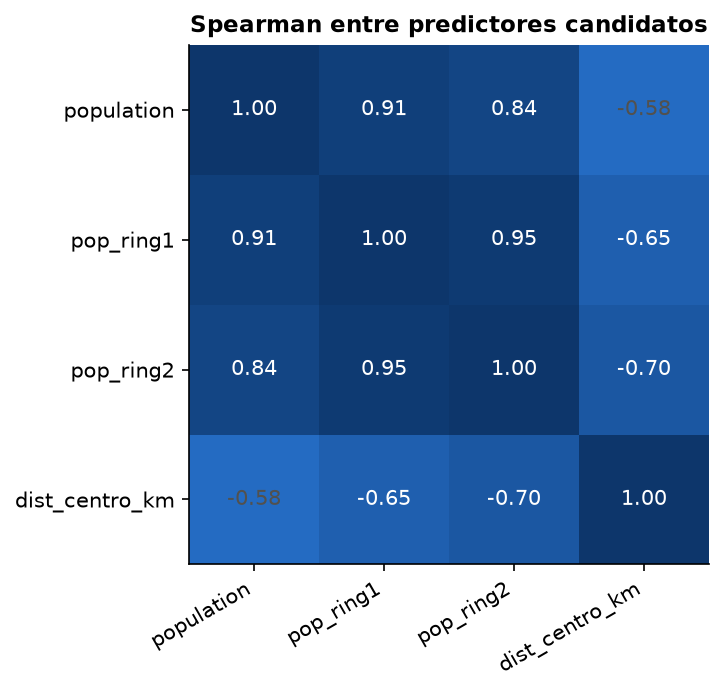
\includegraphics[width=0.5\textwidth]{imagenes/07_desarrollo/7_3_preparacion/correlacion_predictores.png}
  \fuente{Elaboración propia, a partir de
  \var{resultados/03_feature_engineering/correlacion_predictores.csv}.}
\end{figure}

\textbf{Exclusión de la cobertura.} \var{dist_trazado_m} es la distancia del centroide de
la zona al trazado GTFS más cercano, calculada en proyección métrica UTM 19S.
\var{gtfs_covered} vale 1 si esa distancia es de 500~m o menos. Con ese criterio, 634 de
las 1.628 zonas están cubiertas (626 de las 1.381 zonas del modelo). Ambas variables se
excluyen expresamente de los predictores
(secciones~\ref{sec:traduccion-necesidad} y~\ref{sec:area-estudio}), y el notebook de
modelado verifica que ninguna técnica las use. La cobertura se mide contra el trazado y no
contra las paradas, por la naturaleza del paratránsito (sección~\ref{subsec:gtfs}).

Con estas decisiones, el conjunto de predictores queda reducido a dos variables:
\var{dist_centro_km}, que resume la localización, y \var{pop_ring1}, que resume el
entorno. Es un conjunto deliberadamente pequeño. Con 1.381 zonas y una autocorrelación
fuerte, el número efectivo de observaciones independientes es mucho menor que el nominal,
y cada predictor adicional aumenta el riesgo de sobreajuste. Además, ambas variables son
exógenas: ninguna se calcula a partir de las consultas.

\subsection{Conjuntos de entrenamiento y prueba}
\label{sec:conjuntos-entrenamiento-prueba}

El conjunto de prueba se reserva en esta fase, antes de ajustar cualquier modelo, y se usa
una sola vez en la evaluación. La reserva no se hace por zonas individuales sino por
\emph{bloques} H3 de resolución~6: por la autocorrelación documentada en la
sección~\ref{sec:relaciones-variables}, una zona de prueba rodeada de vecinas de
entrenamiento sería casi una copia de ellas, y el error medido resultaría optimista
(sección~\ref{subsec:validacion-espacial}).

Las 1.381 zonas del modelo se reparten en 53 bloques. Para que la prueba represente todo el
gradiente centro-periferia, el sorteo se estratifica por anillo de distancia: en cada
anillo se reserva el 20~\% de sus bloques, con la semilla fija 42. Los cortes entre anillos
(12,52, 18,65 y 22,92~km de la Plaza) son los cuartiles de la distancia media de los
bloques, de modo que cada anillo tiene un número parecido de bloques. El sorteo solo usa la
geometría de los bloques y su anillo: ninguna consulta interviene en la selección.

\begin{table}[H]
  \centering
  \caption{Zonas del modelo por anillo de distancia}
  \label{tab:anillos}
  \interlineadoSimple
  \small
  \begin{tabular}{@{}lrrrrrr@{}}
    \toprule
    \textbf{Anillo} & \textbf{\celda{Distancia\\a la Plaza (km)}} & \textbf{Bloques} & \textbf{\celda{Bloques\\de prueba}} & \textbf{Zonas} & \textbf{Consultas} & \textbf{\celda{Consultas por\\1.000 hab.}} \\
    \midrule
    A1 & hasta 12,52 & 14 & 3 & 501 & 1.854.930 & 2.139,9 \\
    A2 & 12,52 a 18,65 & 13 & 3 & 342 & 66.102 & 303,5 \\
    A3 & 18,65 a 22,92 & 13 & 3 & 234 & 2.251 & 31,9 \\
    A4 & más de 22,92 & 13 & 3 & 304 & 1.053 & 14,9 \\
    \midrule
    Total & & 53 & 12 & 1.381 & 1.924.336 & 1.570,0 \\
    \bottomrule
  \end{tabular}
  \fuente{Elaboración propia, a partir de
  \var{resultados/03_feature_engineering/resumen_anillo.csv} y \var{test_blocks.csv}.}
\end{table}

La tabla~\ref{tab:particion} y la figura~\ref{fig:anillos-prueba} muestran el resultado.
La prueba reúne 12 bloques y 352 zonas (el 25,5~\% de las zonas), pero solo el 9,63~\% de
las consultas.

\begin{table}[H]
  \centering
  \caption{Partición en entrenamiento y prueba por bloques espaciales}
  \label{tab:particion}
  \interlineadoSimple
  \small
  \begin{tabular}{@{}lrrrrr@{}}
    \toprule
    \textbf{Conjunto} & \textbf{Bloques} & \textbf{Zonas} & \textbf{Consultas} & \textbf{Población} & \textbf{\celda{Consultas por\\1.000 hab.}} \\
    \midrule
    Entrenamiento & 41 & 1.029 & 1.738.942 & 908.744 & 1.913,6 \\
    Prueba & 12 & 352 & 185.394 & 316.935 & 585,0 \\
    \bottomrule
  \end{tabular}
  \fuente{Elaboración propia, a partir de
  \var{resultados/03_feature_engineering/particion.csv}.}
\end{table}

\begin{figure}[H]
  \centering
  \caption{Anillos de distancia al centro y bloques reservados como prueba}
  \label{fig:anillos-prueba}
  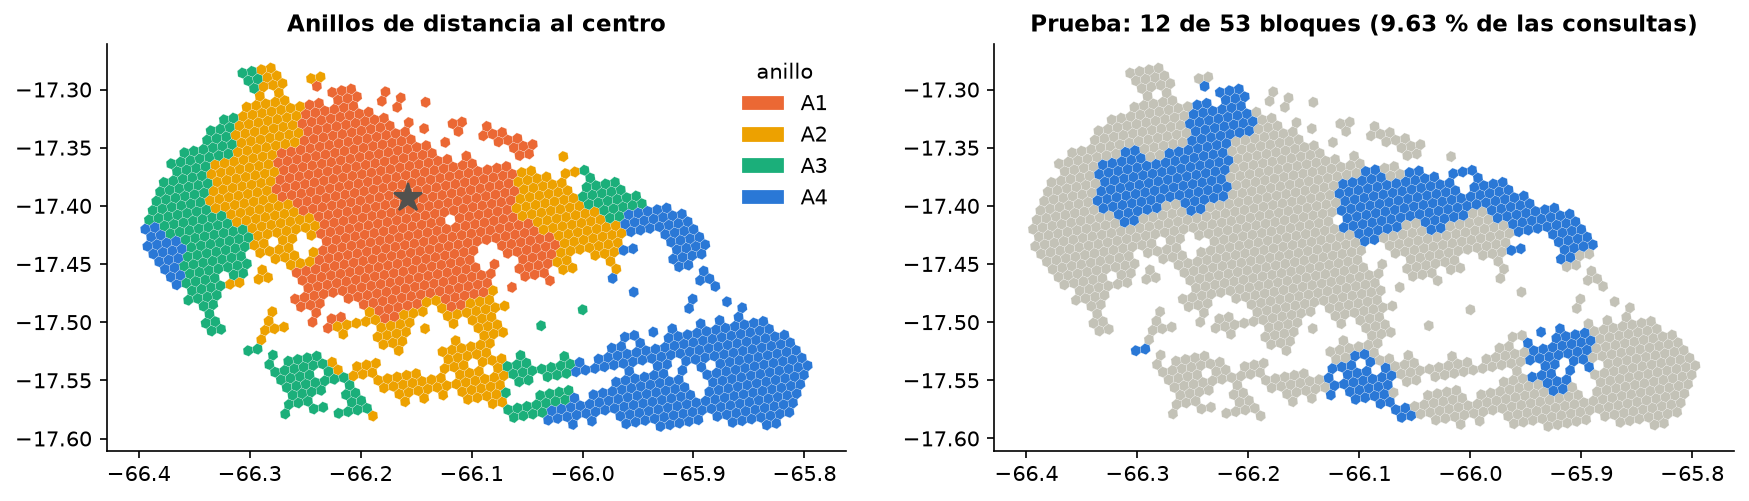
\includegraphics[width=\textwidth]{imagenes/07_desarrollo/7_3_preparacion/anillos_y_prueba.png}
  \fuente{Elaboración propia, a partir de \var{03_feature_engineering} (secciones 8 y 10).
  Izquierda: anillos A1 a A4 (la estrella marca la Plaza 14 de Septiembre); derecha: bloques
  de prueba en azul.}
\end{figure}

El desequilibrio entre zonas y consultas tiene una explicación, y debe tenerse en cuenta
al leer la evaluación. Los bloques del núcleo central, donde se concentra la mayor parte de
las consultas, quedaron del lado de entrenamiento. Por eso la tasa de la prueba (585
consultas por cada 1.000 habitantes) es un tercio de la de entrenamiento (1.913,6). La
prueba es, por tanto, más periférica y menos intensa que el conjunto con el que se
entrena. Es una condición exigente pero realista: la organización necesita estimaciones
confiables justamente en zonas alejadas del centro. Además, 125 de las 352 zonas de prueba
tocan zonas de entrenamiento en el borde de su bloque
(\var{zonas_prueba_borde} en \var{resultados/03_feature_engineering/metricas.json}). Es una
fuga mínima e inevitable en cualquier partición espacial, que se documenta y no se oculta.

El notebook termina con cuatro verificaciones automáticas:
\begin{itemize}
  \item la tabla conserva todas las consultas y no tiene nulos;
  \item los rangos de las variables son válidos;
  \item entrenamiento y prueba no comparten ningún bloque;
  \item ni el objetivo ni las variables GTFS figuran entre los predictores.
\end{itemize}
Los bloques reservados se guardan en \var{test_blocks.csv}. A partir de aquí, el notebook
de modelado solo los descarta y el de evaluación los usa una única vez.

% ============================================================
%  7.4. MODELADO  -- parte del capítulo 7
%  ------------------------------------------------------------
%  Guía 2.7.4: (1) tipo de problema, (2) algoritmos, (3) por qué,
%  (4) entrenamiento, (5) parámetros e hiperparámetros,
%  (6) comparación de alternativas, (7) no presentar un modelo
%  como mejor solo por ser el primero ejecutado.
%  Notebook: 04_modelado.ipynb   Código: src/modelos.py
%  Cifras:   resultados/04_modelado/ (metricas.json, cv_resumen.csv,
%            cv_por_pliegue.csv, regla_seleccion.csv, coeficientes.csv)
% ============================================================
\section{Modelado}
\label{sec:modelado}

El modelado elige la técnica con la que se calcula el conteo esperado de cada zona. Se
ejecuta en el notebook \var{04_modelado} y trabaja solo con las 1.029 zonas de
entrenamiento, repartidas en 41 bloques. Las 352 zonas de prueba se descartan al cargar
los datos y no intervienen en ninguna decisión de esta fase. El protocolo completo, que
incluye las técnicas, los predictores, los pliegues de validación y la regla de selección,
se escribió en \var{config.py} y se registró en el control de versiones antes de ejecutar
el primer modelo.

\subsection{Tipo de problema analítico}
\label{sec:tipo-problema}

Se trata de un problema de \textbf{regresión supervisada sobre datos de conteo con
exposición}, en un corte transversal:
\begin{itemize}
  \item Es \emph{supervisado} porque para cada zona de entrenamiento se conoce el valor
        observado de la variable objetivo, \var{query_count}.
  \item Es una \emph{regresión} porque se estima una cantidad, el número esperado de
        consultas, y no una categoría.
  \item Es un problema de \emph{conteo} porque el objetivo es un entero no negativo, con
        muchos ceros, fuertemente asimétrico y sobredisperso
        (sección~\ref{sec:distribucion-objetivo}). Por eso los errores se miden con la
        devianza de Poisson y no con el error cuadrático (sección~\ref{subsec:devianza-poisson}).
  \item Tiene \emph{exposición} porque, a igualdad de condiciones, el conteo debe crecer en
        proporción a la población. Todas las técnicas estiman, en el fondo, una
        \emph{tasa} de consultas por habitante, que luego se multiplica por la población de
        la zona.
  \item Es \emph{transversal} porque cada zona aporta una sola observación, el total del
        período, y el tiempo no interviene.
\end{itemize}

La predicción se usa de una forma particular: no interesa acertar el conteo de las zonas
de entrenamiento, que ya se conoce, sino obtener para \emph{cada} zona un valor esperado
calculado sin que la zona se vea a sí misma. Ese valor es el que después se compara con lo
observado para medir la brecha (sección~\ref{sec:interpretacion-resultados}).

\subsection{Selección de algoritmos}
\label{sec:seleccion-algoritmos}

Se compararon siete técnicas, ordenadas de menor a mayor complejidad en lo que en este
trabajo se denomina \emph{escalera}. Cada técnica se identifica con un código de letra y
número, que se usa tal cual en el código fuente, los resultados y las figuras:

\begin{itemize}
  \item La letra \textbf{B} viene de \emph{baseline}, que en español se traduce como
    \textbf{línea base}: un \emph{punto de referencia inicial}, es decir, una estimación
    deliberadamente simple que cualquier técnica más elaborada debe superar para justificar
    su complejidad. Las cuatro líneas base (B0 a B3) no ajustan parámetros por optimización.
    Calculan una tasa de consultas por habitante con una regla aritmética y la multiplican
    por la población de la zona.
  \item La letra \textbf{M} viene de \emph{modelo}. Designa las tres técnicas (M1 a M3) que
    estiman parámetros optimizando una función de pérdida o de verosimilitud a partir de
    los predictores \var{dist_centro_km} y \var{pop_ring1}.
  \item El \textbf{número} indica la posición en la escalera: B0 es la más simple y M3 la
    más compleja. Cuando dos técnicas empatan en desempeño, la regla de selección elige la
    de número menor (sección~\ref{sec:regla-seleccion}).
\end{itemize}

La tabla~\ref{tab:escalera-tecnicas} resume las siete técnicas. En todas las fórmulas,
$Y_i$ es el conteo observado de la zona~$i$, $P_i$ su población y $\hat{\mu}_i$ su conteo
esperado. Las sumas se calculan solo sobre zonas de entrenamiento.

\begin{table}[H]
  \centering
  \caption{Escalera de técnicas: códigos, cálculo del esperado y fundamento}
  \label{tab:escalera-tecnicas}
  \interlineadoSimple
  \small
  \begin{tabularx}{\textwidth}{@{}L{0.07\textwidth}L{0.20\textwidth}YL{0.11\textwidth}@{}}
    \toprule
    \textbf{Código} & \textbf{Nombre} & \textbf{Cómo calcula el conteo esperado de una zona} & \textbf{Marco} \\
    \midrule
    B0 & Tasa global & Tasa única de todo el entrenamiento: $\hat{\mu}_i = P_i \cdot \sum Y / \sum P$ & \ref{subsec:lineas-base} \\
    B1 & Tasa por municipio & Tasa del municipio de la zona; si el municipio no está en el entrenamiento, tasa global & \ref{subsec:lineas-base} \\
    B2 & Tasa por anillo & Tasa del anillo de distancia (A1 a A4) de la zona & \ref{subsec:lineas-base} \\
    B3 & Vecindad H3 & Tasa conjunta de las zonas de entrenamiento más cercanas (al menos 3, sin la propia zona) & \ref{subsec:suavizado-vecindad} \\
    M1 & Poisson con \emph{offset} & $\log \hat{\mu}_i = \log P_i + \beta_0 + \beta_1\,d_i + \beta_2 \log(1 + R_i)$, por máxima verosimilitud & \ref{subsec:glm-poisson} \\
    M2 & Binomial negativa NB2 & Igual que M1, con varianza $\mu + \alpha\mu^2$; $\alpha$ se estima con los datos & \ref{subsec:binomial-negativa} \\
    M3 & \emph{Gradient boosting} con pérdida de Poisson & Suma de árboles de decisión sobre $d_i$ y $\log(1+R_i)$, ajustados a la tasa $Y_i/P_i$ con peso $P_i$ & \ref{subsec:gradient-boosting} \\
    \bottomrule
  \end{tabularx}
  \fuente{Elaboración propia, a partir de \var{src/modelos.py} y \var{config.py}. $d_i$:
  \var{dist_centro_km}; $R_i$: \var{pop_ring1}.}
\end{table}

A continuación se explica cada técnica en palabras, tal como está implementada.

\textbf{B0, tasa global.} Supone que todas las zonas tienen la misma propensión a
consultar y que solo difieren en población. Suma las consultas de todas las zonas de
entrenamiento, las divide por su población total y aplica esa tasa única a cada zona. Es
el punto de referencia principal del proyecto (sección~\ref{subsec:modelo-referencia}): si
ninguna técnica lo supera, el contexto territorial no aporta nada más allá de la
población, y la brecha sería una simple comparación de tasas brutas.

\textbf{B1, tasa por municipio.} Calcula una tasa separada para cada municipio con las
zonas de entrenamiento de ese municipio y la aplica a las zonas del mismo municipio.
Representa la hipótesis de que la propensión a consultar cambia de un municipio a otro,
por ejemplo por diferencias de adopción o de cobertura cartográfica. Si una zona pertenece
a un municipio sin zonas de entrenamiento, recibe la tasa global.

\textbf{B2, tasa por anillo.} Hace lo mismo que B1, pero con los cuatro anillos de
distancia a la Plaza. Representa el gradiente centro-periferia de la economía urbana
(sección~\ref{subsec:lineas-base}).

\textbf{B3, vecindad H3.} Estima la tasa de una zona con la tasa conjunta de sus vecinas de
entrenamiento más cercanas. El procedimiento tiene tres pasos:
\begin{enumerate}
  \item Se buscan zonas de entrenamiento en el primer anillo H3 alrededor de la zona, sin
        incluirla a ella.
  \item Si hay menos de tres, se amplía la búsqueda al segundo anillo, luego al tercero, y
        así hasta un máximo de diez anillos.
  \item Con las vecinas encontradas se calcula $\sum Y_j / \sum P_j$, y ese cociente se
        multiplica por la población de la zona. Si ni siquiera a diez anillos hay tres
        vecinas de entrenamiento, se usa la tasa global.
\end{enumerate}
El umbral de tres vecinas (\var{VECINAS_MIN}) evita que la tasa dependa de una sola zona
vecina. El límite de diez anillos (\var{K_VECINDAD_MAX}), unos 9~km, impide usar zonas
demasiado lejanas. B3 aprovecha directamente la autocorrelación espacial hallada en la
sección~\ref{sec:relaciones-variables}. No estima coeficientes: su ``ajuste'' consiste en
memorizar los conteos y las poblaciones de entrenamiento, como un estimador de vecinos
cercanos. Como la zona nunca entra en su propio cálculo, el esperado de B3 no puede copiar
el valor observado.

\textbf{M1, regresión de Poisson con offset.} Es un modelo lineal generalizado con enlace
logarítmico. El término $\log P_i$ entra con coeficiente fijo igual a 1 (\emph{offset}),
de modo que el modelo describe cómo varía la \emph{tasa} por habitante con la distancia al
centro y con la población del entorno. Los coeficientes se estiman por máxima
verosimilitud. La relación es multiplicativa: cada kilómetro de distancia multiplica la
tasa por $e^{\beta_1}$. M1 supone que la varianza del conteo es igual a su media.

\textbf{M2, binomial negativa NB2.} Mantiene la misma ecuación para la media que M1, pero
permite que la varianza crezca más rápido que la media, según $\mu + \alpha\mu^2$. El
parámetro de sobredispersión $\alpha$ se estima con los datos: si $\alpha = 0$, M2 se
reduce a M1. Responde al hallazgo de que la varianza es decenas de miles de veces la media
(sección~\ref{sec:distribucion-objetivo}).

\textbf{M3, gradient boosting con pérdida de Poisson.} Construye una suma de árboles de
decisión, cada uno de los cuales corrige los errores de los anteriores. Así captura
relaciones no lineales e interacciones entre la distancia y la población del entorno sin
especificarlas de antemano. La implementación usada no admite \emph{offset}, así que se
modela la tasa $Y_i/P_i$ ponderando cada zona por su población, una formulación
equivalente en esperanza (sección~\ref{subsec:gradient-boosting}). Sus hiperparámetros se
eligen con una validación interna, descrita en la sección~\ref{sec:hiperparametros}.

\subsection{Justificación de la selección}
\label{sec:justificacion-algoritmos}

Las siete técnicas no se eligieron por exhaustividad, sino para que cada peldaño ponga a
prueba \emph{una} hipótesis adicional sobre qué determina las consultas esperadas. La
tabla~\ref{tab:hipotesis-escalera} explicita esa lógica y el hallazgo de la
sección~\ref{sec:comprension-datos} que motiva cada peldaño.

\begin{table}[H]
  \centering
  \caption{Hipótesis que pone a prueba cada peldaño de la escalera}
  \label{tab:hipotesis-escalera}
  \interlineadoSimple
  \small
  \begin{tabularx}{\textwidth}{@{}L{0.08\textwidth}YL{0.33\textwidth}@{}}
    \toprule
    \textbf{Código} & \textbf{Hipótesis que añade} & \textbf{Hallazgo que la motiva} \\
    \midrule
    B0 & La población basta para explicar las consultas & Spearman de 0,855 entre conteo y población \\
    B1 & La tasa difiere entre municipios & Cercado: 86~\% de las consultas con 51~\% de la población \\
    B2 & La tasa decae con la distancia al centro & Spearman de $-0{,}68$ entre tasa y distancia \\
    B3 & Zonas cercanas tienen tasas parecidas & $I$ de Moran de 0,72 entre vecinas \\
    M1 & La tasa varía de forma continua con la distancia y el entorno & Asociación de la tasa con \var{pop_ring1} y \var{dist_centro_km} \\
    M2 & Además, la varianza excede a la media & Varianza 46.569 veces la media \\
    M3 & Además, la relación es no lineal o tiene interacciones & Dispersión grande entre zonas de población similar \\
    \bottomrule
  \end{tabularx}
  \fuente{Elaboración propia, a partir de las secciones~\ref{sec:distribucion-objetivo}
  y~\ref{sec:relaciones-variables}.}
\end{table}

Ordenar las técnicas de esta forma permite interpretar la comparación. Si un peldaño mejora
claramente al anterior, su hipótesis aporta información. Si no lo mejora, la complejidad
añadida no se justifica. Incluir líneas base simples no es un trámite: en datos con
autocorrelación fuerte y pocas unidades independientes, un estimador local sencillo puede
competir con modelos más elaborados, y solo compararlos en las mismas condiciones permite
saberlo.

La escalera tampoco incluye bosques aleatorios u otras variantes de \emph{boosting}: M3
representa a la familia de conjuntos de árboles, y M2 a la de modelos que relajan el
supuesto de Poisson.

Tampoco se incluyeron modelos con exceso de ceros (ZIP y ZINB), pese a estar mencionados en
la sección~\ref{subsec:binomial-negativa}. La razón es empírica y la muestra la
tabla~\ref{tab:ceros-esperados}: en entrenamiento hay 345 ceros observados. El modelo de
Poisson espera 631,5, casi el doble; la binomial negativa espera 323,8, prácticamente los
observados (razón de 0,94). En otras palabras, una vez corregida la sobredispersión no queda
un exceso de ceros que modelar.

\begin{table}[H]
  \centering
  \caption{Ceros observados y esperados en las zonas de entrenamiento}
  \label{tab:ceros-esperados}
  \interlineadoSimple
  \small
  \begin{tabular}{@{}lrrrr@{}}
    \toprule
    \textbf{Técnica} & \textbf{\celda{Ceros\\observados}} & \textbf{\celda{Ceros\\esperados}} & \textbf{\celda{Esperados /\\observados}} & \textbf{\celda{Zonas con\\$\hat{\mu} < 0{,}5$}} \\
    \midrule
    B3 vecindad H3 & 345 & --- & --- & 179 \\
    M1 Poisson & 345 & 631,5 & 1,83 & 625 \\
    M2 binomial negativa & 345 & 323,8 & 0,94 & 89 \\
    \bottomrule
  \end{tabular}
  \fuente{Elaboración propia, a partir de \var{resultados/04_modelado/ceros_esperados.csv}
  (1.029 zonas de entrenamiento). B3 no define una distribución de probabilidad, por lo que
  no tiene ceros esperados.}
\end{table}

Los ceros del proyecto son, en su mayoría, muestrales y no estructurales. Son zonas
pobladas donde el evento no se observó, pero donde podría ocurrir si la aplicación
ofreciera información útil. Modelarlos con un proceso aparte absorbería justamente la señal
que el proyecto busca interpretar como brecha. Además, M2, que corrige la sobredispersión,
no fue seleccionada por la regla de un error estándar
(sección~\ref{sec:regla-seleccion}), de modo que un ZIP no tendría base empírica para
justificar su complejidad adicional.

\subsection{Proceso de entrenamiento}
\label{sec:proceso-entrenamiento}

Las siete técnicas se entrenan y comparan con una \textbf{validación cruzada espacial por
bloques}. Los 41 bloques de entrenamiento se reparten en cinco pliegues con
\var{GroupKFold}, un procedimiento que asigna cada bloque \emph{entero} a un solo pliegue.
Cada pliegue reúne entre 205 y 207 zonas. El proceso se repite cinco veces:
\begin{enumerate}
  \item Se toman cuatro pliegues como entrenamiento y el quinto como validación.
  \item Cada técnica se ajusta solo con los cuatro pliegues de entrenamiento. Todo lo que
        se estima (tasas, coeficientes, $\alpha$ e hiperparámetros) ocurre dentro de ese
        ajuste.
  \item Cada técnica predice las zonas del pliegue de validación, que no ha visto.
  \item Se calculan las métricas de ese pliegue.
\end{enumerate}

Al terminar, cada zona de entrenamiento tiene una predicción \emph{fuera de pliegue} por
cada técnica, calculada por un modelo que no la vio. La validación replica así la situación
real de uso, que es estimar zonas cuyas consultas no se conocen. Como los pliegues se forman
por bloques de unos 36~km\textsuperscript{2}, una zona de validación no tiene vecinas
inmediatas en el entrenamiento salvo en el borde de su bloque. Esto importa especialmente
para B3, que de otro modo tomaría la tasa de vecinas casi idénticas.

Una vez aplicada la regla de selección, la técnica elegida se ajusta con las 1.029 zonas
de entrenamiento y se guarda (\var{modelo_final.joblib}). Ese modelo final es el único que
se aplica a la prueba (sección~\ref{sec:evaluacion-resultados}).

El notebook termina con tres verificaciones:
\begin{itemize}
  \item ninguna zona de prueba intervino en la validación;
  \item cada zona de entrenamiento se predijo exactamente una vez por técnica, con bloques
        completos;
  \item los predictores usados son solo \var{dist_centro_km} y \var{pop_ring1}.
\end{itemize}

\subsection{Parámetros e hiperparámetros}
\label{sec:hiperparametros}

La tabla~\ref{tab:parametros-protocolo} reúne los parámetros del protocolo. Todos se
fijaron antes de modelar y ninguno se ajustó después de ver los resultados.

\begin{table}[H]
  \centering
  \caption{Parámetros del protocolo de modelado}
  \label{tab:parametros-protocolo}
  \interlineadoSimple
  \small
  \begin{tabularx}{\textwidth}{@{}L{0.30\textwidth}L{0.17\textwidth}Y@{}}
    \toprule
    \textbf{Parámetro (\var{config.py})} & \textbf{Valor} & \textbf{Significado} \\
    \midrule
    \var{PLIEGUES} & 5 & Pliegues de la validación cruzada por bloque \\
    \var{TOLERANCIA_EE} & 1,0 & Tolerancia de la regla de selección, en errores estándar \\
    \var{VECINAS_MIN} & 3 & B3: mínimo de zonas vecinas de entrenamiento \\
    \var{K_VECINDAD_MAX} & 10 & B3: anillo H3 máximo antes de usar la tasa global \\
    \var{GRILLA_GB} & 8 combinaciones & M3: profundidad máxima $\in \{3, \text{sin límite}\}$; mínimo de zonas por hoja $\in \{20, 50\}$; tasa de aprendizaje $\in \{0{,}05;\ 0{,}1\}$ \\
    \var{PLIEGUES_INTERNOS_GB} & 3 & M3: pliegues por bloque de la validación interna \\
    Iteraciones de M3 & hasta 300 & Con parada temprana \\
    \var{SEMILLA} & 42 & Semilla única del proyecto \\
    \bottomrule
  \end{tabularx}
  \fuente{Elaboración propia, a partir de \var{config.py} y \var{src/modelos.py}.}
\end{table}

\textbf{Hiperparámetros de M3.} M3 es la única técnica con hiperparámetros propiamente
dichos, y se eligen mediante \emph{validación anidada}. Dentro del ajuste de cada pliegue
externo, sus zonas de entrenamiento se dividen a su vez en tres pliegues internos por
bloque. Para cada una de las ocho combinaciones de la grilla se calcula la devianza media
interna, y se elige la menor. Así, la elección de hiperparámetros nunca ve el pliegue
externo de validación.

Los hiperparámetros elegidos por M3 en cada pliegue quedan registrados en
\var{cv_hiperparametros_m3.csv} (tabla~\ref{tab:hiperparametros-m3}). En el ajuste
completo sobre las 1.029 zonas de entrenamiento, la combinación elegida es: profundidad sin
límite, al menos 20 zonas por hoja y tasa de aprendizaje de 0,05, con 83 iteraciones tras
la parada temprana.

\begin{table}[H]
  \centering
  \caption{Hiperparámetros elegidos por M3 en cada pliegue y en el ajuste completo}
  \label{tab:hiperparametros-m3}
  \interlineadoSimple
  \small
  \begin{tabular}{@{}lrrrrr@{}}
    \toprule
    \textbf{Ajuste} & \textbf{\celda{Profundidad\\máxima}} & \textbf{\celda{Mínimo de\\zonas por hoja}} & \textbf{\celda{Tasa de\\aprendizaje}} & \textbf{Iteraciones} & \textbf{\celda{Devianza\\interna}} \\
    \midrule
    Pliegue 0 & 3 & 50 & 0,10 & 63 & 2.828,6 \\
    Pliegue 1 & 3 & 20 & 0,10 & 57 & 2.221,9 \\
    Pliegue 2 & 3 & 20 & 0,10 & 30 & 1.449,9 \\
    Pliegue 3 & 3 & 20 & 0,10 & 78 & 2.266,7 \\
    Pliegue 4 & sin límite & 20 & 0,10 & 33 & 2.389,4 \\
    \midrule
    Ajuste completo & sin límite & 20 & 0,05 & 83 & 2.172,3 \\
    \bottomrule
  \end{tabular}
  \fuente{Elaboración propia, a partir de
  \var{resultados/04_modelado/cv_hiperparametros_m3.csv} y \var{metricas.json}
  (\var{m3_*}). Devianza interna: media de los tres pliegues internos de la combinación
  elegida.}
\end{table}

La tabla muestra que la combinación elegida no es estable. En cuatro de los cinco pliegues
gana la profundidad 3 con tasa de 0,10, y el número de iteraciones varía entre 30 y 78. El
ajuste completo, en cambio, prefiere árboles sin límite de profundidad y una tasa menor.
Esa variabilidad es coherente con la inestabilidad de M3 entre pliegues de validación
(tabla~\ref{tab:cv-pliegues}): con dos predictores y pocos bloques independientes, pequeños
cambios en el conjunto de entrenamiento alteran la configuración óptima. Esta inestabilidad
es una razón más para no elegir por la menor media: con diferencias de desempeño menores que
la variabilidad entre pliegues, la regla conservadora de un error estándar
(sección~\ref{sec:regla-seleccion}) protege de premiar una técnica por azar de la partición.

La parada temprana de M3 reserva el 10~\% de las zonas al azar, no por bloques. La medición
de esa reserva muestra que el 98,6~\% de las zonas reservadas tiene una vecina en el resto
del entrenamiento (\var{pct_reserva_parada_con_vecina}). Eso introduce una fuga mínima
dentro de cada pliegue interno, de modo que la validación interna puede ser optimista. La
limitación se documenta en la sección~\ref{sec:limitaciones}. No afecta a la comparación
entre técnicas: la validación externa por bloques, con la que se aplica la regla de
selección, no depende de esa reserva.

\textbf{Parámetros estimados de M1 y M2.} La tabla~\ref{tab:coeficientes} presenta los
coeficientes estimados con las 1.029 zonas de entrenamiento.

\begin{table}[H]
  \centering
  \caption{Coeficientes de los modelos de Poisson (M1) y binomial negativa (M2)}
  \label{tab:coeficientes}
  \interlineadoSimple
  \small
  \begin{tabular}{@{}lrr@{}}
    \toprule
    \textbf{Parámetro} & \textbf{M1 Poisson} & \textbf{M2 binomial negativa} \\
    \midrule
    Intercepto $\beta_0$ & $-0{,}804$ & $-3{,}261$ \\
    \var{dist_centro_km} ($\beta_1$) & $-0{,}625$ & $-0{,}133$ \\
    $\log(1 + \text{\var{pop_ring1}})$ ($\beta_2$) & $0{,}406$ & $0{,}401$ \\
    Sobredispersión $\alpha$ & --- & $2{,}630$ \\
    \bottomrule
  \end{tabular}
  \fuente{Elaboración propia, a partir de \var{resultados/04_modelado/coeficientes.csv}.}
\end{table}

Los coeficientes se interpretan en escala multiplicativa:
\begin{itemize}
  \item En M2, cada kilómetro adicional de distancia a la Plaza multiplica la tasa esperada
        por $e^{-0{,}133} \approx 0{,}88$, es decir, la reduce en torno a un 12~\%. En M1 la
        reducción es mucho más brusca ($e^{-0{,}625} \approx 0{,}54$ por kilómetro).
  \item En ambos modelos, un aumento del 10~\% en la población del entorno eleva la tasa en
        torno a un 4~\% (elasticidad de 0,40).
\end{itemize}

La diferencia en el efecto de la distancia tiene una explicación. M1 pondera cada zona
según su conteo, y las zonas centrales, con decenas de miles de consultas, dominan el
ajuste. M2, al permitir más varianza en los conteos altos, reparte el peso de forma más
uniforme entre centro y periferia.

La sobredispersión se confirma con dos indicadores. El estadístico de dispersión de
Pearson del modelo M1, que debería valer cerca de 1 si el supuesto de Poisson se
cumpliera, alcanza 62.143.817,5. El parámetro $\alpha = 2{,}63$ de M2 está muy lejos de
cero.

\subsection{Comparación de alternativas}
\label{sec:comparacion-alternativas}

La tabla~\ref{tab:cv-resumen} presenta el desempeño de las siete técnicas en la validación
cruzada. La métrica principal, declarada de antemano, es la devianza de Poisson media entre
pliegues (sección~\ref{subsec:devianza-poisson}): cuanto menor, mejor. Las demás columnas
ayudan a interpretar el resultado:
\begin{itemize}
  \item $D^2$ es la fracción de la devianza explicada frente a predecir la media del
        pliegue (sección~\ref{subsec:d2});
  \item el Spearman mide si la técnica ordena bien las zonas;
  \item la calibración fuera de pliegue divide la suma de lo esperado entre la suma de lo
        observado en las 1.029 zonas (sección~\ref{subsec:calibracion}).
\end{itemize}

\begin{table}[H]
  \centering
  \caption{Resultados de la validación cruzada espacial por técnica}
  \label{tab:cv-resumen}
  \interlineadoSimple
  \small
  \begin{tabular}{@{}lrrrrr@{}}
    \toprule
    \textbf{Técnica} & \textbf{\celda{Devianza\\media}} & \textbf{DE} & \textbf{\celda{$D^2$\\medio}} & \textbf{\celda{Spearman\\medio}} & \textbf{Calibración} \\
    \midrule
    B0 tasa global & 5.676,1 & 6.645,8 & $-2{,}00$ & 0,825 & 0,922 \\
    B1 tasa por municipio & 5.665,3 & 5.577,0 & $-1{,}57$ & 0,695 & 0,879 \\
    B2 tasa por anillo & 4.742,7 & 5.579,3 & $-1{,}50$ & 0,793 & 0,903 \\
    \textbf{B3 vecindad H3} & \textbf{1.389,3} & \textbf{1.944,1} & \textbf{0,73} & \textbf{0,799} & \textbf{0,977} \\
    M1 Poisson & 994,6 & 1.172,3 & 0,73 & 0,772 & 0,807 \\
    M2 binomial negativa & 4.190,1 & 7.098,8 & 0,46 & 0,843 & 0,354 \\
    M3 \emph{gradient boosting} & 2.265,9 & 4.200,1 & 0,73 & 0,840 & 0,641 \\
    \bottomrule
  \end{tabular}
  \fuente{Elaboración propia, a partir de \var{resultados/04_modelado/cv_resumen.csv}. DE:
  desviación estándar entre los cinco pliegues. Spearman medio: media de los cinco valores
  por pliegue. Calibración: fuera de pliegue, sobre las 1.029 zonas.}
\end{table}

\begin{figure}[H]
  \centering
  \caption{Devianza de Poisson media de cada técnica y umbral de la regla de selección}
  \label{fig:comparacion-tecnicas}
  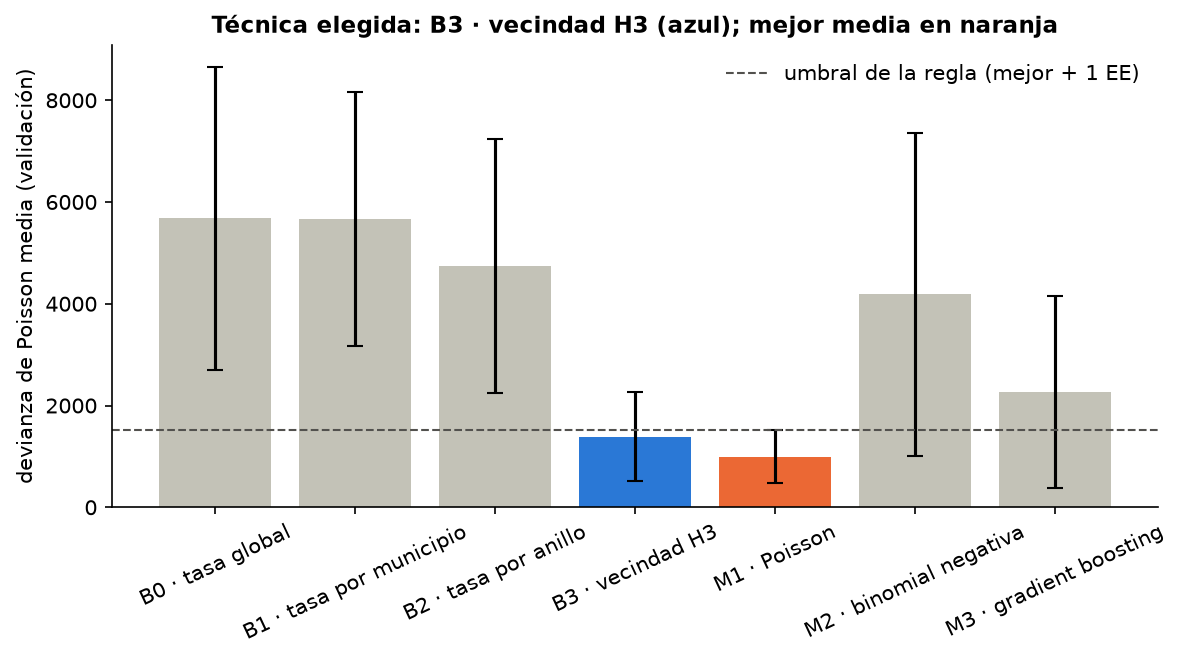
\includegraphics[width=0.72\textwidth]{imagenes/07_desarrollo/7_4_modelado/comparacion_tecnicas.png}
  \fuente{Elaboración propia, a partir de \var{04_modelado} (sección 6). Barras de error:
  $\pm 1$ error estándar; línea discontinua: umbral de la regla (mejor media más un error
  estándar); azul: técnica elegida; naranja: menor devianza media.}
\end{figure}

La tabla y la figura~\ref{fig:comparacion-tecnicas} permiten cinco lecturas:
\begin{enumerate}
  \item \textbf{Las líneas base por grupo apenas mejoran a la tasa global.} B1 y B2 tienen
        devianzas similares a B0, y su $D^2$ medio es negativo. En promedio predicen peor
        que la media del propio pliegue: una tasa común a todo un municipio o anillo no
        distingue entre zonas vecinas con comportamientos muy distintos.
  \item \textbf{La vecindad produce el mayor salto de la escalera.} B3 reduce la devianza
        de 4.743 a 1.389 y lleva el $D^2$ a 0,73. La información local es mucho más útil
        que las agrupaciones administrativas o por distancia.
  \item \textbf{M1 obtiene la menor devianza media (994,6)}, con un $D^2$ igual al de B3.
        Sin embargo, su calibración es de 0,807: en conjunto subestima el total de
        consultas en torno a un 19~\%.
  \item \textbf{M2 y M3 no compensan su complejidad.} M2 ordena bien las zonas (Spearman de
        0,843), pero su calibración de 0,354 indica que estima apenas un tercio del volumen
        real. Al corregir la sobredispersión da menos peso a las zonas de conteo alto,
        precisamente donde está casi todo el volumen. M3 alcanza un buen $D^2$ medio, pero
        su devianza es muy inestable entre pliegues.
  \item \textbf{La variabilidad entre pliegues es alta.} Las desviaciones estándar son del
        mismo orden que las medias. La tabla~\ref{tab:cv-pliegues} muestra la causa.
\end{enumerate}

\begin{table}[H]
  \centering
  \caption{Devianza de Poisson por pliegue de validación}
  \label{tab:cv-pliegues}
  \interlineadoSimple
  \small
  \begin{tabular}{@{}lrrrrr@{}}
    \toprule
    \textbf{Técnica} & \textbf{Pliegue 0} & \textbf{Pliegue 1} & \textbf{Pliegue 2} & \textbf{Pliegue 3} & \textbf{Pliegue 4} \\
    \midrule
    B0 & 2.811,7 & 3.914,3 & 17.477,0 & 2.510,8 & 1.666,5 \\
    B1 & 2.100,2 & 7.009,3 & 14.898,9 & 2.319,5 & 1.998,9 \\
    B2 & 2.274,0 & 2.886,6 & 14.697,3 & 2.052,4 & 1.803,1 \\
    B3 & 155,7 & 1.491,2 & 4.722,5 & 128,3 & 448,7 \\
    M1 & 145,5 & 1.199,8 & 2.956,3 & 241,8 & 429,6 \\
    M2 & 322,1 & 3.376,8 & 16.663,5 & 271,0 & 316,9 \\
    M3 & 107,2 & 971,0 & 9.753,8 & 147,5 & 349,9 \\
    \bottomrule
  \end{tabular}
  \fuente{Elaboración propia, a partir de \var{resultados/04_modelado/cv_por_pliegue.csv}.}
\end{table}

El pliegue 2 contiene bloques del centro de la ciudad, con conteos de decenas de miles de
consultas por zona, y su devianza es varias veces mayor que la de los demás en todas las
técnicas. Es ahí donde M3 falla más (9.753,8), probablemente porque sus árboles no
extrapolan bien a zonas con valores de los predictores poco frecuentes en el
entrenamiento de ese pliegue. En los pliegues periféricos (0, 3 y 4), B3, M1 y M3 tienen
errores de magnitud parecida. Esta heterogeneidad es la razón por la que la selección no
puede basarse solo en la media: la diferencia entre dos técnicas debe juzgarse frente a
la incertidumbre de esa media.

\subsection{Regla de selección}
\label{sec:regla-seleccion}

La técnica final se elige con una regla escrita en el protocolo antes de ejecutar ningún
modelo, conocida como \textbf{regla de un error estándar}: \emph{se elige la técnica más
simple de la escalera cuya devianza media no supere la mejor devianza media más un error
estándar de esta.}

El \emph{error estándar} (EE) mide cuánto podría variar la devianza media si los pliegues
fueran otros. Se calcula como la desviación estándar entre pliegues dividida por la raíz
del número de pliegues: $\text{EE} = \text{DE} / \sqrt{5}$. Dos técnicas cuyas medias
difieren menos de un EE no pueden distinguirse con los datos disponibles. En ese caso, la
regla prefiere la más simple, porque tiene menos supuestos, es más fácil de explicar y es
menos propensa al sobreajuste. La tabla~\ref{tab:regla-seleccion} aplica la regla.

\begin{table}[H]
  \centering
  \caption{Aplicación de la regla de un error estándar}
  \label{tab:regla-seleccion}
  \interlineadoSimple
  \small
  \begin{tabular}{@{}lrrcc@{}}
    \toprule
    \textbf{Técnica} & \textbf{\celda{Devianza\\media}} & \textbf{EE} & \textbf{\celda{$\leq$ umbral\\(1.518,8)}} & \textbf{Resultado} \\
    \midrule
    B0 & 5.676,1 & 2.972,1 & no & --- \\
    B1 & 5.665,3 & 2.494,1 & no & --- \\
    B2 & 4.742,7 & 2.495,1 & no & --- \\
    \textbf{B3} & \textbf{1.389,3} & \textbf{869,4} & \textbf{sí} & \textbf{elegida} \\
    M1 & 994,6 & 524,3 & sí & mejor media \\
    M2 & 4.190,1 & 3.174,7 & no & --- \\
    M3 & 2.265,9 & 1.878,3 & no & --- \\
    \bottomrule
  \end{tabular}
  \fuente{Elaboración propia, a partir de \var{resultados/04_modelado/regla_seleccion.csv}.
  Umbral $= 994{,}6 + 1{,}0 \times 524{,}3 = 1.518{,}8$.}
\end{table}

La mejor devianza media es la de M1 (994,6), con un error estándar de 524,3, lo que fija el
umbral en 1.518,8. Solo dos técnicas quedan por debajo: M1 y B3 (1.389,3). Como B3 ocupa
una posición anterior en la escalera, la regla \textbf{elige B3, el suavizado por vecindad
H3}.

La elección no responde a que B3 haya sido la primera técnica ejecutada ni a que tenga el
menor error. Las siete técnicas se evaluaron en las mismas condiciones y M1 obtuvo una
media menor. Se elige B3 porque la regla declarada de antemano establece que una diferencia
de 395 unidades de devianza, inferior a un error estándar, no justifica un modelo
paramétrico con supuestos que los propios datos contradicen, como la varianza igual a la
media. Hay además dos indicios, que no forman parte de la regla, a favor de B3 en el uso
previsto:
\begin{itemize}
  \item su calibración fuera de pliegue es de 0,977, frente a 0,807 de M1, de modo que
        reproduce mejor el volumen total;
  \item ordena las zonas algo mejor: calculado sobre todas las predicciones fuera de pliegue
        juntas, el Spearman es de 0,802 frente a 0,760. Estas cifras difieren de las de la
        tabla~\ref{tab:cv-resumen} (0,799 y 0,772), que son la media de los cinco valores
        calculados pliegue a pliegue.
\end{itemize}

La figura~\ref{fig:calibracion-oof} compara las predicciones fuera de pliegue de ambas
técnicas con lo observado.

\begin{figure}[H]
  \centering
  \caption{Observado frente a esperado fuera de pliegue: B3 y M1}
  \label{fig:calibracion-oof}
  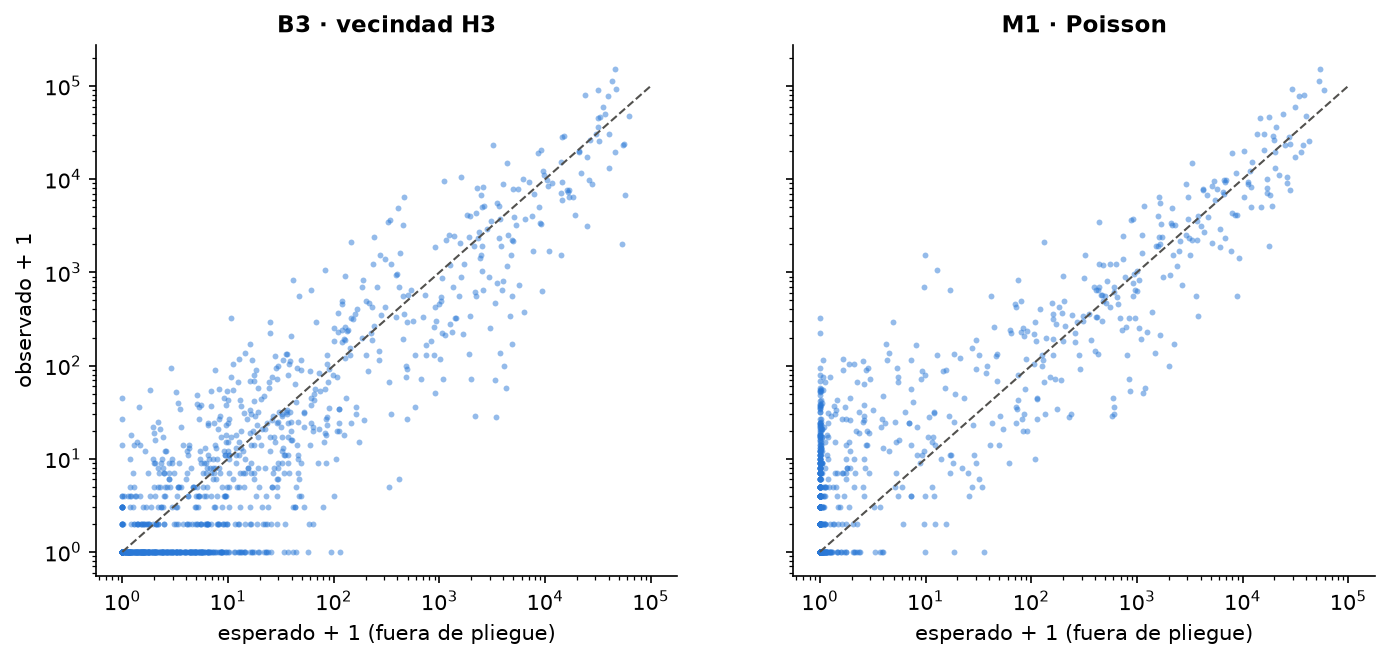
\includegraphics[width=0.9\textwidth]{imagenes/07_desarrollo/7_4_modelado/calibracion_oof.png}
  \fuente{Elaboración propia, a partir de \var{04_modelado} (sección 6). Ambos ejes en
  escala logarítmica (valor $+1$); la diagonal marca la coincidencia exacta.}
\end{figure}

Las dos nubes siguen la diagonal en los conteos altos, pero difieren en los bajos. B3
asigna a las zonas sin consultas esperados pequeños y variados, tomados de sus vecinas. M1
acumula muchas zonas con esperado cercano a cero, que en la columna izquierda aparecen con
conteos observados de hasta cientos de consultas. Esa diferencia es relevante para el
problema: una técnica que asigna esperado casi nulo a una zona no puede detectar en ella
una brecha negativa.

La técnica elegida tiene también un límite: B3 aprende de los vecinos, así que las zonas
que conviven con un polo de actividad heredan una tasa muy alta. Sus consecuencias se
examinan en la evaluación.

% ============================================================
%  7.5. EVALUACIÓN Y RESULTADOS  -- parte del capítulo 7
%  ------------------------------------------------------------
%  Archivo separado para que cada fase de CRISP-DM se pueda
%  editar y compilar por separado. Solo contenido: el formato,
%  los rótulos y las referencias los resuelve el preámbulo.
%  Los \label originales se conservan sin cambios.
% ============================================================
\section{Evaluación y Resultados}
\label{sec:evaluacion-resultados}

Esta sección documenta la quinta fase de CRISP-DM, ejecutada mediante cinco scripts
(\var{21_hypothesis_tests.py} a \var{28_ranking_explainer.py}) sobre las
predicciones de los cuatro modelos de la sección~\ref{sec:modelado}.

\subsection{Métricas y resultados por modelo}
\label{sec:resultados-modelo}

Se reportan tres métricas, cada una con un rol distinto dado que el objetivo es fuertemente
asimétrico (sección~\ref{sec:seleccion-algoritmos}): el \textbf{MAE} (error absoluto medio),
interpretable directamente en consultas por semana; el \textbf{RMSE}, que penaliza más los
errores grandes y es por tanto sensible a la presencia de valores extremos; y el
\textbf{R\textsuperscript{2}}, la proporción de varianza explicada respecto de predecir
siempre la media.

\begin{table}[htbp]
  \centering
  \caption{Desempeño comparado en el conjunto de prueba (8 semanas nunca vistas)}
  \label{tab:resultados-modelos}
  \interlineadoSimple
  \begin{tabular}{lrrr}
    \toprule
    \textbf{Modelo} & \textbf{MAE} & \textbf{RMSE} & \textbf{R\textsuperscript{2}} \\
    \midrule
    \textbf{Random Forest (final)} & \textbf{10,19} & \textbf{80,70} & \textbf{0,656} \\
    Base estacional (media móvil 4 sem.) & 11,05 & 85,70 & 0,613 \\
    Base ingenua (persistencia, $t-1$) & 11,30 & 91,90 & 0,555 \\
    XGBoost & 13,85 & 102,82 & 0,442 \\
    Lasso & 44,03 & 520,76 & $-13,305$ \\
    Ridge & 48,97 & 559,13 & $-15,491$ \\
    \bottomrule
  \end{tabular}
  \fuente{Elaboración propia, a partir de \var{19_model_comparison.py} ---
  \var{reports/03_modeling/02_model_comparison.md}.}
\end{table}

\begin{figure}[htbp]
  \centering
  \caption{Predicho vs. observado, Random Forest, conjunto de prueba}
  \label{fig:pred-vs-obs}
  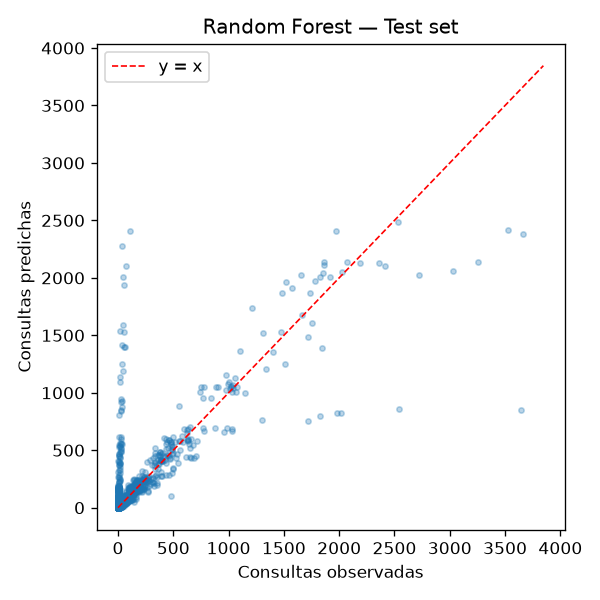
\includegraphics[width=0.7\textwidth]{imagenes/fig_pred_vs_obs_rf.png}
  \fuente{Elaboración propia, a partir de \var{19_model_comparison.py}.}
\end{figure}

\subsubsection{Hallazgo: inestabilidad de extrapolación de los modelos lineales}

Ridge y Lasso muestran R\textsuperscript{2} fuertemente negativo en prueba pese a un ajuste
razonable en entrenamiento (MAE de 30,06 y 25,57 respectivamente): 50 y 42 de las 12.416
predicciones de cada uno alcanzan el techo de seguridad de extrapolación impuesto sobre la
reversión \texttt{expm1} (sección~\ref{sec:tipo-problema}). La causa es la combinación de una
tendencia sostenida --\var{week_idx} toma en prueba valores nunca vistos en
entrenamiento-- con la asimetría extrema del objetivo (Gini~$=0{,}934$,
sección~\ref{sec:sensibilidad-h3}): un pequeño error en escala logarítmica se amplifica
exponencialmente al revertir la transformación. \textbf{No es un defecto de implementación:
es evidencia de que la relación entre demanda y condiciones territoriales no es lineal.} Los
modelos de árboles no sufren este problema porque sus predicciones están acotadas por los
valores observados en las hojas de entrenamiento.

\subsection{Sobreajuste y subajuste}
\label{sec:sobreajuste}

\begin{table}[htbp]
  \centering
  \caption{Brecha entre entrenamiento y prueba (MAE)}
  \label{tab:brecha-train-test}
  \interlineadoSimple
  \begin{tabular}{lrrr}
    \toprule
    \textbf{Modelo} & \textbf{MAE entrenamiento} & \textbf{MAE prueba} & \textbf{Brecha} \\
    \midrule
    Random Forest & 2,19 & 10,19 & $+8,00$ \\
    XGBoost & 2,09 & 13,85 & $+11,76$ \\
    Lasso & 25,57 & 44,03 & $+18,46$ \\
    Ridge & 30,06 & 48,97 & $+18,92$ \\
    \bottomrule
  \end{tabular}
  \fuente{Elaboración propia, a partir de \var{19_model_comparison.py}.}
\end{table}

La brecha de Random Forest ($+8{,}00$) es menor que la de XGBoost ($+11{,}76$) pese a
hiperparámetros de complejidad similar, señal de menor sobreajuste relativo. Las curvas de
aprendizaje --Random Forest reentrenado con tamaños de entrenamiento crecientes, evaluado
contra una ventana de validación de 13 semanas no vista-- refuerzan esta lectura.

\begin{figure}[htbp]
  \centering
  \caption{Curva de aprendizaje de Random Forest}
  \label{fig:curva-aprendizaje}
  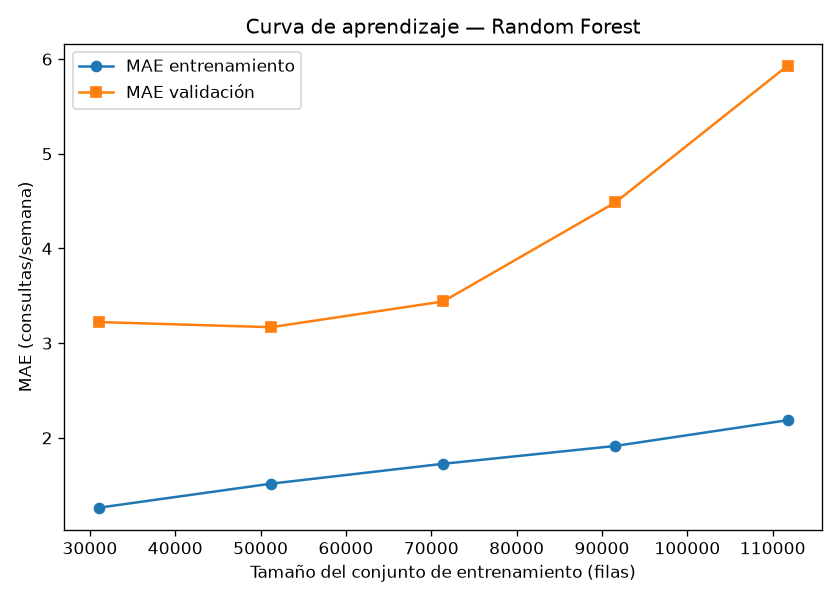
\includegraphics[width=0.7\textwidth]{imagenes/fig_learning_curve.png}
  \fuente{Elaboración propia, a partir de \var{23_error_analysis.py} ---
  \var{reports/04_evaluation/03_error_analysis.md}.}
\end{figure}

La brecha entrenamiento-validación crece de forma moderada a medida que aumenta el tamaño de
entrenamiento ($+1{,}96 \to +1{,}65 \to +1{,}71 \to +2{,}57 \to +3{,}74$), con un MAE de
entrenamiento que se mantiene bajo (1,26 a 2,19) mientras el de validación oscila en un rango
razonable (3,2 a 5,9): la firma esperada de un árbol de profundidad acotada
(\var{max_depth}$=10$) que ajusta ruido de forma limitada, sin señal de varianza
descontrolada. La curva tiene solo cinco puntos por costo computacional --cada uno reentrena
un modelo completo--, suficiente para descartar sobreajuste severo pero no para un
diagnóstico fino.

\subsection{Contraste de hipótesis}
\label{sec:contraste-hipotesis}

\subsubsection{H1 --- Brecha de cobertura centro-periferia}

Se contrasta si las celdas periféricas (mayor distancia al centro) tienen una tasa de
demanda no resuelta (\var{pct_uncovered_orig}) significativamente mayor que las
centrales. La unidad de análisis es la \textbf{celda}, no la celda-semana: se promedia
\var{pct_uncovered_orig} sobre todas las semanas de cada celda, porque tratar cada
semana como observación independiente constituiría pseudorreplicación --inflaría el tamaño
muestral de 1.552 a decenas de miles y produciría un valor p espuriamente pequeño. Los
grupos se definen por la mediana de \var{dist_center_km} (15,49~km): 776 celdas
centrales y 776 periféricas, un corte simple y documentado pero arbitrario, que no
corresponde a ningún límite administrativo real.

\begin{table}[htbp]
  \centering
  \caption{Contraste H1: tasa de demanda no resuelta por grupo territorial}
  \label{tab:h1-resultado}
  \interlineadoSimple
  \begin{tabular}{lrr}
    \toprule
    \textbf{Grupo} & \textbf{n celdas} & \textbf{Media \var{pct_uncovered_orig}} \\
    \midrule
    Central & 776 & 0,213 \\
    Periferia & 776 & 0,351 \\
    \bottomrule
  \end{tabular}
  \fuente{Elaboración propia, a partir de \var{21_hypothesis_tests.py} ---
  \var{reports/04_evaluation/01_hypothesis_tests.md}.}
\end{table}

La prueba de Shapiro-Wilk rechazó la normalidad en ambos grupos ($p=2{,}18\times10^{-41}$ en
el centro, $p=1{,}423\times10^{-38}$ en la periferia) --resultado esperable, dado que la
variable es una proporción con masa concentrada en 0 y 1--, lo que fundamenta el uso de la
prueba U de Mann-Whitney, no paramétrica. El resultado es concluyente: estadístico
$341{.}618{,}0$, $p=6{,}101\times10^{-9}$, significativo a $\alpha=0{,}05$, con una
correlación biserial por rangos de $-0{,}135$ (tamaño de efecto pequeño, dado el tamaño
muestral). \textbf{Se confirma H1}: las celdas periféricas tienen una tasa de demanda no
resuelta significativamente mayor que las centrales.

\subsubsection{H2 --- Random Forest frente a la línea base estacional}

Se contrasta si el error del modelo final es significativamente menor que el de la media
móvil de 4 semanas. El test de Diebold-Mariano, diseñado específicamente para comparar
exactitud predictiva entre dos modelos sobre una serie temporal, opera sobre la serie
semanal de 8 puntos de prueba: con esa potencia insuficiente por construcción, el resultado
no es significativo (estadístico $-0{,}705$, $p=0{,}503$). Un resultado no significativo no
implica equivalencia entre los modelos, solo que ocho semanas no alcanzan para distinguirlos
con confianza; la ventana de prueba se fijó en la sección~\ref{sec:particion-cronologica}
para preservar datos de entrenamiento, no para maximizar la potencia de este contraste.

Se complementa con una prueba de Wilcoxon de rangos con signo, pareada por celda (1.552
observaciones, potencia suficiente): estadístico $287.045{,}0$, $p=0{,}0326$, significativo.
A primera vista esto contradice que Random Forest solo supere a la base en el 31,0~\% de las
celdas; la explicación está en la magnitud, no en el conteo:

\begin{table}[htbp]
  \centering
  \caption{Dónde gana cada método (test de Wilcoxon pareado por celda)}
  \label{tab:h2-desglose}
  \interlineadoSimple
  \begin{tabularx}{\textwidth}{@{}Xrrr@{}}
    \toprule
    \textbf{Grupo} & \textbf{n celdas} & \textbf{Dif. media (RF $-$ base)} & \textbf{Demanda media} \\
    \midrule
    Gana Random Forest & 481 & $-3,72$ & 42,9 consultas/sem. \\
    Gana la base estacional & 632 & $+0,71$ & 13,8 consultas/sem. \\
    Empate exacto & 439 & --- & --- \\
    \bottomrule
  \end{tabularx}
  \fuente{Elaboración propia, a partir de \var{21_hypothesis_tests.py}.}
\end{table}

Random Forest gana por un margen grande en celdas de alta demanda y pierde por un margen
pequeño en celdas casi sin actividad. \textbf{Se confirma H2, con matices}: la ventaja de
Random Forest sobre la línea base es estadísticamente significativa y está concentrada
exactamente en las celdas de mayor demanda --el segmento operativamente más relevante--, no
distribuida de manera uniforme. Reportar solo el valor p o solo el porcentaje de celdas
ganadas habría sido engañoso en direcciones opuestas.

\subsection{Análisis de errores}
\label{sec:analisis-errores}

La media de residuos de Random Forest en prueba es $-4{,}758$. Esta cifra no debe calificarse
de sesgo despreciable: representa cerca de la mitad del MAE de prueba (10,19), lo que indica
una tendencia sistemática a la sobrepredicción, atribuible en buena parte a las semanas
parciales que se describen a continuación.

\begin{figure}[htbp]
  \centering
  \caption{Distribución de residuos por celda, conjunto de prueba}
  \label{fig:residuos}
  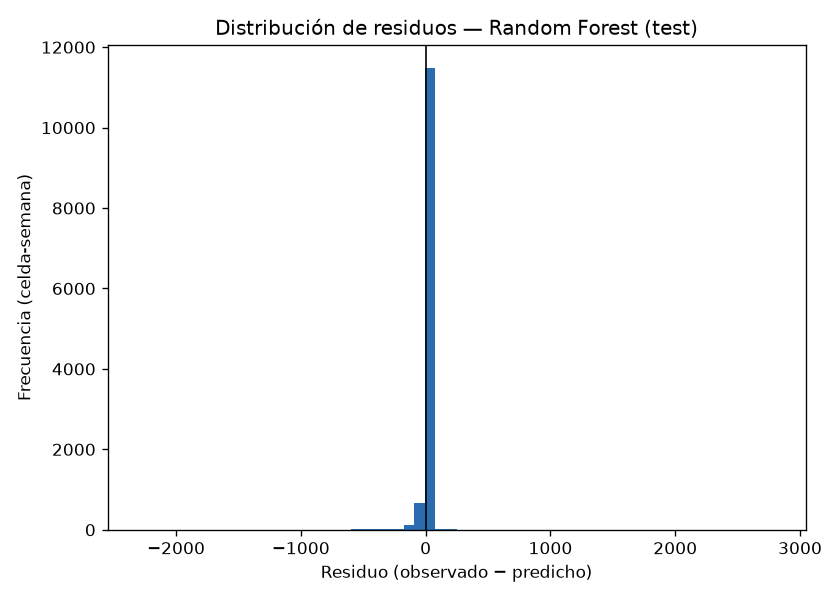
\includegraphics[width=0.65\textwidth]{imagenes/fig_residuals_by_cell.png}
  \fuente{Elaboración propia, a partir de \var{23_error_analysis.py}.}
\end{figure}

\subsubsection{Hallazgo: dos semanas de prueba son fragmentos de un día}
\label{sec:semanas-parciales}

Al construir la serie semanal agregada se detectó que la demanda observada total cae a
apenas 1--3~\% de una semana normal en dos de las ocho semanas de prueba: 2024-W18 (909
consultas, la semana de reanudación tras el vacío, con solo unas 5 horas de datos) y
2024-W23 (1.367 consultas, el corte final del dataset, con solo unas 11 horas de datos). No
se trata de semanas con demanda real más baja sino de fragmentos de un solo día --un
artefacto de cobertura de exportación no advertido al fijar la partición
(sección~\ref{sec:particion-cronologica}).

\begin{table}[htbp]
  \centering
  \caption{Impacto de las semanas parciales sobre las métricas del modelo final}
  \label{tab:semanas-parciales}
  \interlineadoSimple
  \begin{tabular}{lrrr}
    \toprule
    \textbf{Escenario} & \textbf{MAE} & \textbf{RMSE} & \textbf{R\textsuperscript{2}} \\
    \midrule
    Las 8 semanas de prueba (resultado principal) & 10,19 & 80,70 & 0,656 \\
    Las 6 semanas completas (sin las parciales) & 5,91 & 52,87 & 0,889 \\
    \bottomrule
  \end{tabular}
  \fuente{Elaboración propia, a partir de \var{23_error_analysis.py} ---
  \var{reports/04_evaluation/03_error_analysis.md}.}
\end{table}

Esta monografía reporta \textbf{ambas cifras juntas}, y no una sola. El MAE de 10,19 se
mantiene como resultado principal por ser la evaluación más conservadora y no requerir una
decisión de exclusión posterior a la observación de los datos; el MAE de 5,91 es la
estimación más representativa del desempeño en una semana calendario completa, y es
consistente con el historial de validación cruzada (2,8 a 6,2,
sección~\ref{sec:hiperparametros}), frente al cual 10,19 resulta atípico una vez comprendida
su causa. Presentar solo la segunda cifra sería selección posterior favorable; presentar solo
la primera ocultaría que el error está inflado por un artefacto identificado y rastreado
hasta el dato crudo.

\begin{figure}[htbp]
  \centering
  \caption{Estabilidad temporal del error semanal en el conjunto de prueba}
  \label{fig:estabilidad-error}
  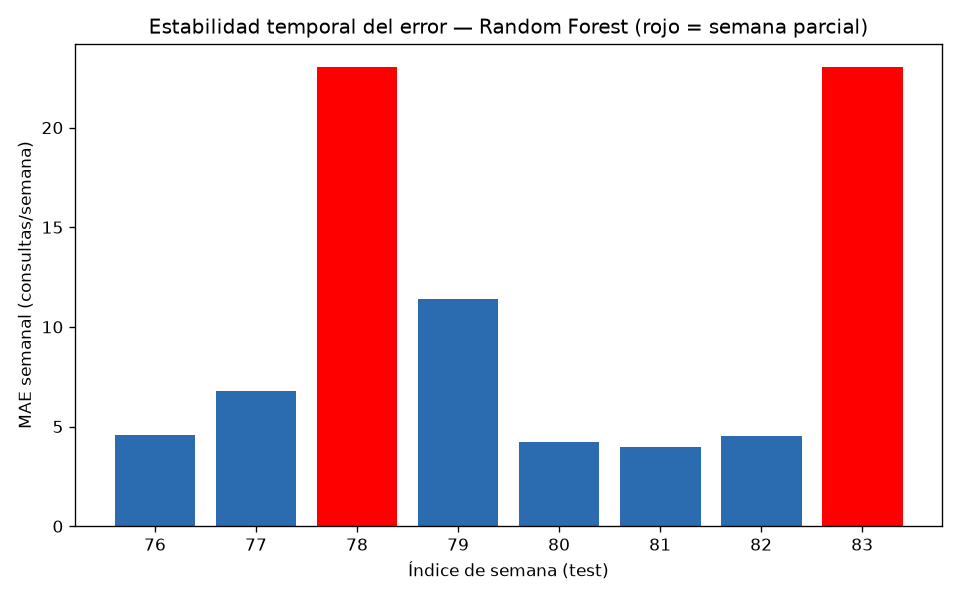
\includegraphics[width=0.7\textwidth]{imagenes/fig_weekly_error_stability.png}
  \fuente{Elaboración propia, a partir de \var{23_error_analysis.py}. Las semanas
  2024-W18 y 2024-W23 (parciales) se resaltan.}
\end{figure}

El artefacto no se limita a las dos semanas donde se originó: 2024-W19, la semana
inmediatamente posterior a 2024-W18, también registra un MAE elevado (11,38, más del doble de
la mediana de las semanas limpias) pese a no tener ningún problema de datos propio, porque
hereda de 2024-W18 un \var{lag1_n_queries_orig} artificialmente bajo (909 consultas en
vez de un nivel normal de más de 40.000). El horizonte de pronóstico evaluado no muestra
degradación progresiva por sí solo; la única inestabilidad detectada tiene una causa puntual
e identificada, no un problema estructural del modelo.

\subsection{Interpretación desde el problema original}
\label{sec:interpretacion-resultados}

La pregunta de investigación --cómo se distribuye la demanda de información de transporte no
resuelta y qué características del territorio se asocian con esa distribución-- se responde
con evidencia convergente de tres análisis. Primero, H1 confirma estadísticamente que la
brecha de cobertura es mayor en la periferia. Segundo, el gradiente espacial de demanda es
real: la correlación de Spearman entre \var{dist_center_km} y la demanda decae tanto
para la demanda observada ($\rho=-0{,}615$, $p=2{,}8\times10^{-162}$) como para la predicha
($\rho=-0{,}618$, $p=3{,}3\times10^{-164}$).

\begin{figure}[htbp]
  \centering
  \caption{Demanda semanal observada vs. distancia al centro}
  \label{fig:demanda-distancia}
  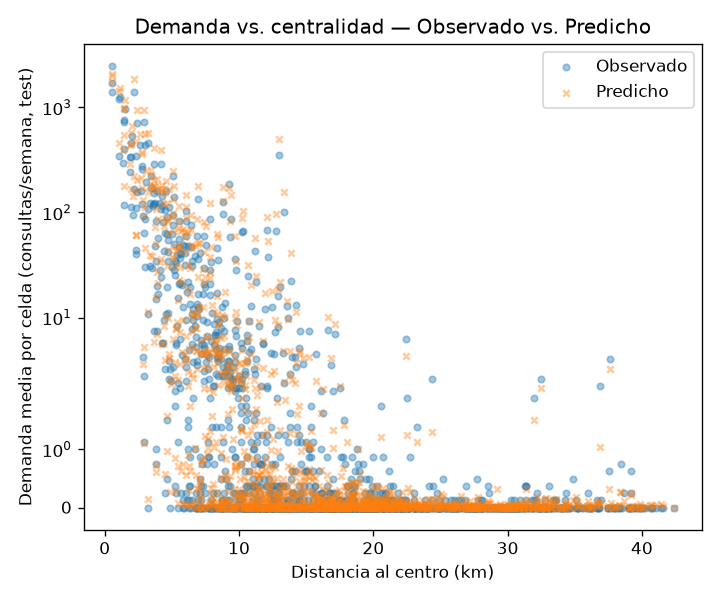
\includegraphics[width=0.7\textwidth]{imagenes/fig_demand_vs_distance.png}
  \fuente{Elaboración propia, a partir de \var{22_results_analysis.py} ---
  \var{reports/04_evaluation/02_results_analysis.md}.}
\end{figure}

Tercero, H2 muestra que el valor predictivo del modelo está concentrado exactamente donde
más importa operativamente: las celdas de mayor demanda. En conjunto, la periferia combina
\textbf{menor demanda absoluta} con \textbf{peor cobertura relativa} --un patrón consistente
con zonas de expansión urbana con transporte formal insuficiente, y no con una simple falta
de interés de los usuarios; debe recordarse, como se ha señalado en capítulos anteriores, que
``demanda'' significa aquí consultas de planificación --intención de viaje-- y no
desplazamientos confirmados.

\begin{figure}[htbp]
  \centering
  \caption{Demanda semanal agregada, observada vs. predicha (conjunto de prueba)}
  \label{fig:demanda-semanal}
  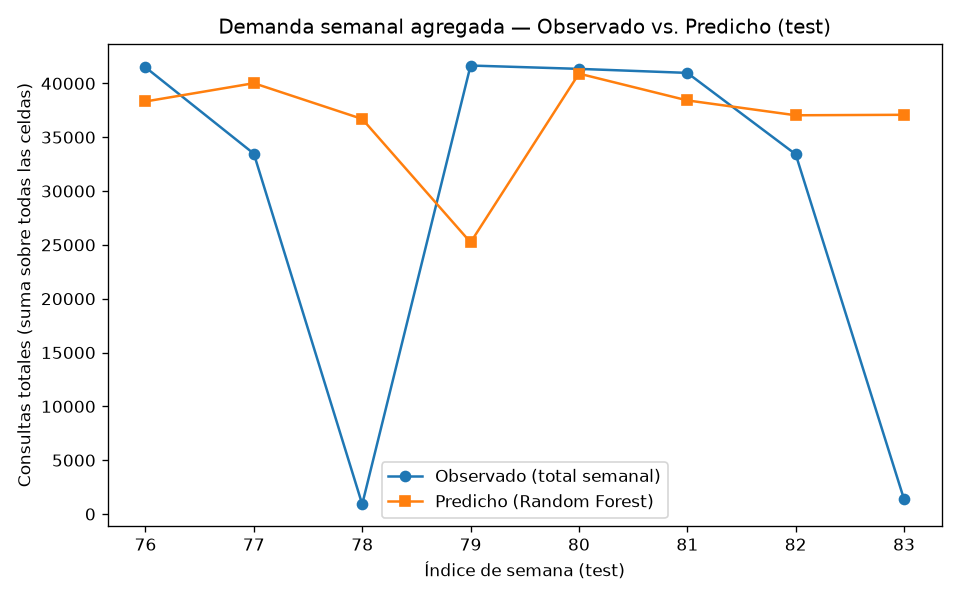
\includegraphics[width=0.7\textwidth]{imagenes/fig_weekly_demand_test.png}
  \fuente{Elaboración propia, a partir de \var{22_results_analysis.py}. Las semanas
  2024-W18 y 2024-W23 (parciales, sección~\ref{sec:semanas-parciales}) explican los mayores
  desvíos agregados de la serie.}
\end{figure}

\subsubsection{Importancia de variables}
\label{sec:importancia-variables}

Las variables autorregresivas dominan la importancia en Random Forest y XGBoost
(\var{roll_mean4_n_queries_orig} explica el 97,9~\% de la reducción de impureza en
Random Forest), coherente con la fuerte autocorrelación semanal de la demanda documentada en
la sección~\ref{sec:cobertura-temporal}.

\begin{figure}[htbp]
  \centering
  \caption{Importancia de variables (Gini), Random Forest}
  \label{fig:importancia-rf}
  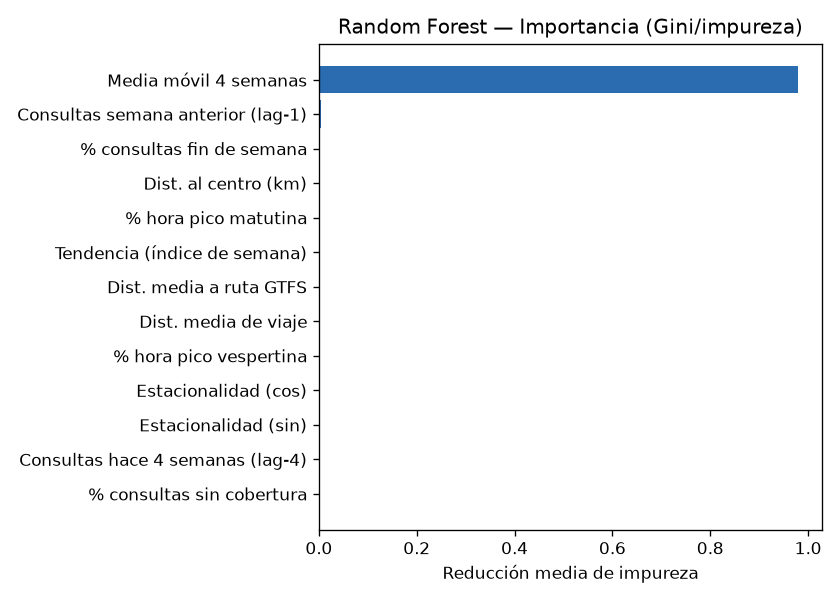
\includegraphics[width=0.65\textwidth]{imagenes/fig_feature_importance_rf.png}
  \fuente{Elaboración propia, a partir de \var{20_feature_importance.py} ---
  \var{reports/03_modeling/03_feature_importance.md}.}
\end{figure}

La señal territorial es más relevante de lo que sugiere la importancia por ganancia: en
XGBoost, \var{dist_center_km} ocupa la octava posición por ganancia pero asciende al
tercer lugar por magnitud media de SHAP, un método de interpretabilidad que atribuye a cada
variable su contribución marginal a cada predicción individual. Lasso --que lleva 9 de 13
coeficientes a cero, actuando como selector de variables-- conserva precisamente
\var{dist_center_km} (coeficiente estandarizado $-0{,}424$),
\var{roll_mean4_n_queries_orig} ($+0{,}396$), \var{lag1_n_queries_orig}
($+0{,}187$) y \var{pct_uncovered_orig} ($-0{,}077$) como la señal independiente más
robusta, con signos coherentes con H1: mayor distancia al centro y mayor proporción sin
cobertura se asocian con menor demanda.

\subsection{¿Sirve el modelo para priorizar? Un criterio preinscrito, refutado}
\label{sec:sirve-para-priorizar}

Si el modelo no gana por precisión de valor de forma contundente, el argumento operativo que
quedaba era que, aunque no acertara la magnitud exacta, ordenara bien las celdas para efectos
de priorización territorial. Esta sección lo somete a prueba con un criterio \textbf{declarado
antes de observar los resultados}: el modelo sirve para priorizar si ordena mejor que la
media móvil de 4 semanas, con diferencia media positiva, signo consistente entre semanas y
una prueba pareada que no lo contradiga. Declarar el criterio de antemano es lo que distingue
un hallazgo de una racionalización posterior, precisamente porque la comparación podía salir
en contra.

\textbf{El criterio no se cumple.} Promediando sobre las 6 semanas completas de prueba (se
excluyen las semanas parciales de la sección~\ref{sec:semanas-parciales}):

\begin{table}[htbp]
  \centering
  \caption{Métricas de ordenamiento territorial, promedio de las 6 semanas completas de prueba}
  \label{tab:ranking-metricas}
  \interlineadoSimple
  \begin{tabular}{lrrr}
    \toprule
    \textbf{Método} & \textbf{vRecall@20} & \textbf{NDCG@20} & \textbf{$\tau$-b de Kendall} \\
    \midrule
    \textbf{Base: media móvil 4 sem.} & \textbf{0,996} & \textbf{0,999} & \textbf{0,853} \\
    Random Forest & 0,995 & 0,996 & 0,850 \\
    XGBoost & 0,993 & 0,997 & 0,843 \\
    Base: persistencia ($t-1$) & 0,983 & 0,994 & 0,800 \\
    Ranking aleatorio (piso) & 0,022 & 0,104 & 0,001 \\
    \bottomrule
  \end{tabular}
  \fuente{Elaboración propia, a partir de \var{26_ranking_metrics.py} ---
  \var{reports/04_evaluation/04_ranking_metrics.md}.}
\end{table}

Random Forest no supera a la media móvil de 4 semanas en ninguna de las 6 semanas completas,
en ninguna de las métricas de ordenamiento evaluadas: el recuento de volumen alcanzable en
las 20 celdas elegidas (vRecall@20, la métrica principal, continua e insensible a empates), la
calidad del orden ponderada por posición (NDCG@20, calculada sobre relevancia logarítmica
porque con conteos crudos todos los métodos saturan por encima de 0,97) y la correlación de
rangos ($\tau$-b de Kendall, restringida a las celdas con demanda media de entrenamiento
$\geq 5$ para no dejar que domine el 76,6~\% de observaciones con demanda nula en prueba).
Ningún corte rescata la comparación: ni el estrato de demanda media (correlación de Spearman
0,957 contra 0,958 de la base) ni el ranking de los cambios semana a semana (0,458 contra
0,514, también a favor de la base).

\begin{figure}[htbp]
  \centering
  \caption{Comparación de métricas de ordenamiento por método y semana}
  \label{fig:ranking-comparacion}
  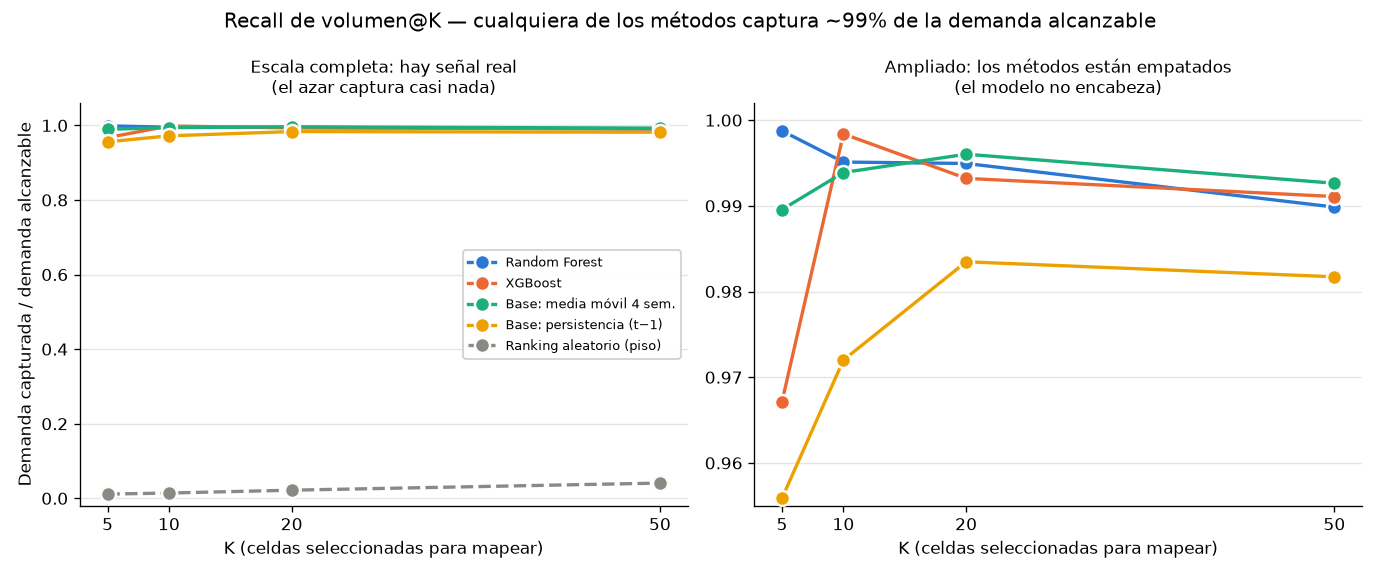
\includegraphics[width=0.75\textwidth]{imagenes/fig_ranking_comparison.png}
  \fuente{Elaboración propia, a partir de \var{26_ranking_metrics.py}.}
\end{figure}

\begin{figure}[htbp]
  \centering
  \caption{Cómo se calcula e interpreta la métrica de priorización}
  \label{fig:ranking-explicador}
  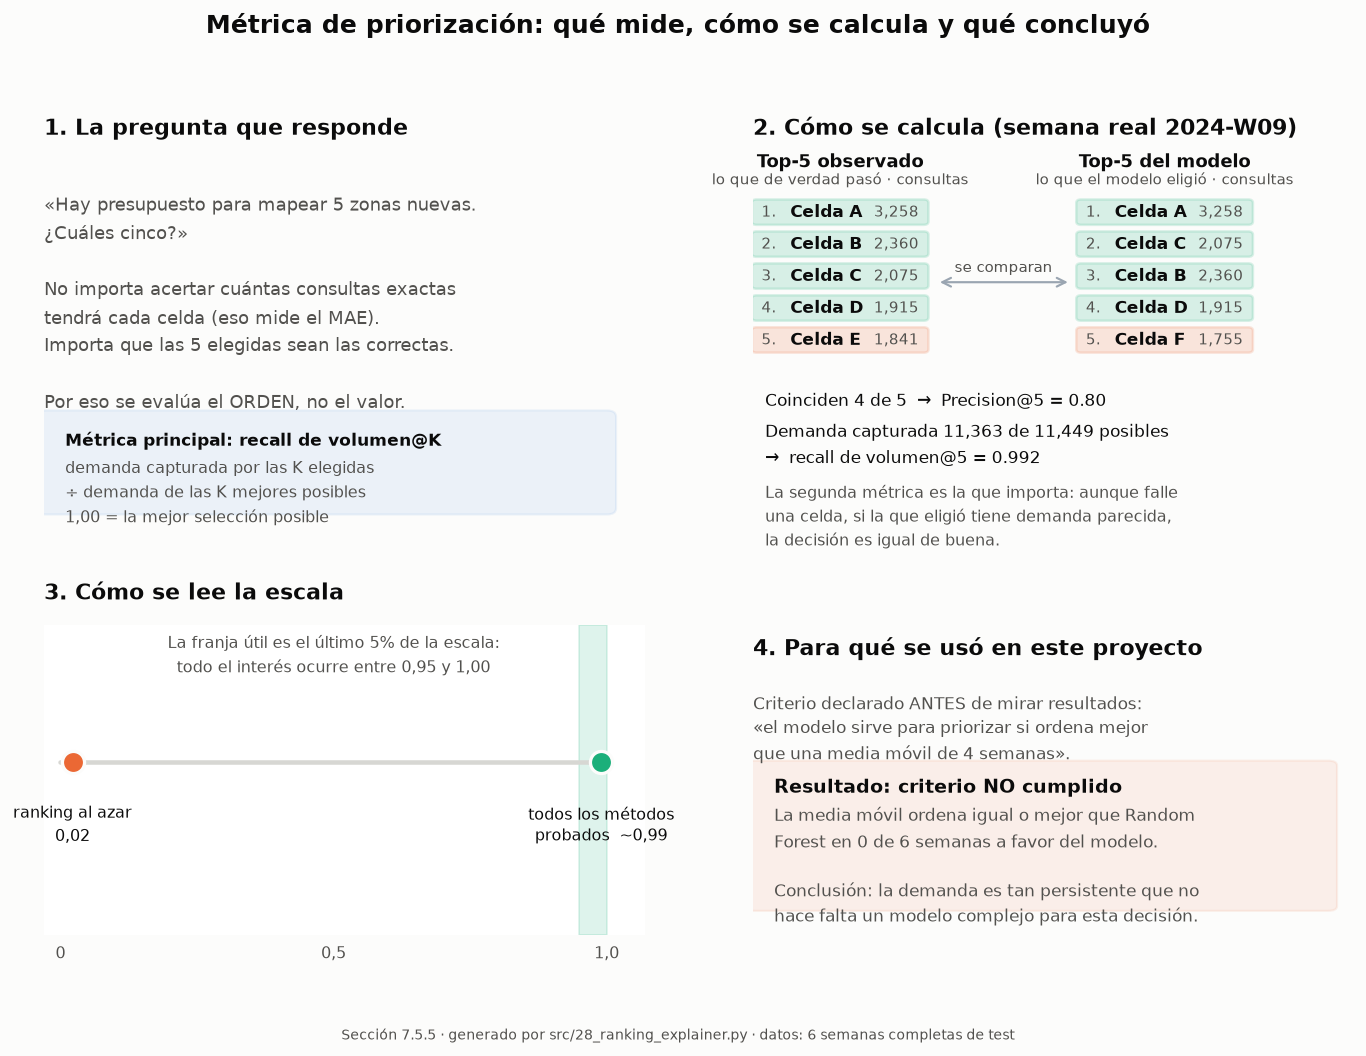
\includegraphics[width=0.75\textwidth]{imagenes/fig_ranking_explainer.png}
  \fuente{Elaboración propia, a partir de \var{28_ranking_explainer.py}.}
\end{figure}

Un coeficiente de correlación de rangos alto --como el $\rho=0{,}877$ entre demanda
observada y predicha reportado en la sección~\ref{sec:interpretacion-resultados}-- es fácil
de obtener cuando la distribución subyacente está tan concentrada como aquí (Gini$=0{,}934$,
sección~\ref{sec:sensibilidad-h3}): el ordenamiento de celdas es casi invariante entre
semanas, de modo que cualquier estimador --incluida una media móvil, e incluso la
persistencia-- reproduce ese orden. Esa cifra mide que el modelo no destruye una señal
trivialmente disponible; no mide que aporte capacidad de ordenamiento propia, que es
justamente lo que esta comparación contra competencia refuta.

\textbf{Este resultado no debilita el trabajo, lo fortalece.} Se obtuvo con un criterio
declarado de antemano y una comparación que podía salir en contra, exactamente lo que
distingue un hallazgo de una racionalización posterior. La formulación correcta es que, para
decidir qué celdas mapear a un horizonte de una semana, no se justifica un modelo complejo:
una media móvil de cuatro semanas ordena igual o mejor, y es además transparente, barata de
operar y auditable. La contribución de este trabajo está en el pipeline reproducible, la
caracterización territorial y el diagnóstico de cobertura (H1), no en la superioridad de un
estimador de valor. El alcance de esta refutación es específico: vale para horizonte de una
semana; a horizontes mayores la media móvil envejece y el modelo podría mostrar ventaja, pero
esa prueba no se realizó --requeriría reconstruir los rezagos y reentrenar-- y queda
declarada como pendiente, no como ventaja supuesta.

\subsection{Selección y justificación del modelo final}
\label{sec:seleccion-final}

\textbf{Random Forest se selecciona como modelo final}, con un criterio explícito aplicado
en el siguiente orden: menor MAE de prueba entre los cuatro modelos ajustados (10,19); menor
brecha entre entrenamiento y prueba que XGBoost ($+8{,}00$ frente a $+11{,}76$); y único
modelo que supera de forma consistente a ambas líneas base. XGBoost se descarta pese a un MAE
de validación cruzada competitivo (4,17 frente a 3,58 de Random Forest): en el conjunto de
prueba resulta peor (13,85) que la propia línea base estacional (11,05) --un caso concreto de
por qué no debe elegirse un modelo por su posición en una única métrica de validación. Haber
sido el primer modelo ejecutado no cuenta como criterio, exigencia explícita de la guía de la
materia.

La selección se sostiene también en interpretabilidad y costo computacional: Random Forest no
requiere las precauciones de extrapolación que exigirían Ridge o Lasso en producción, y su
tiempo de entrenamiento es compatible con la cadencia de reentrenamiento trimestral propuesta
en la sección~\ref{sec:despliegue}. Su ventaja frente a la línea base es real y
estadísticamente significativa donde más importa operativamente (H2), aunque --como se
estableció en la sección~\ref{sec:sirve-para-priorizar}-- esa ventaja no se traduce en una
mejor capacidad de ordenamiento territorial que una media móvil simple.

% ============================================================
%  7.6. DESPLIEGUE  -- parte del capítulo 7
%  ------------------------------------------------------------
%  Archivo separado para que cada fase de CRISP-DM se pueda
%  editar y compilar por separado. Solo contenido: el formato,
%  los rótulos y las referencias los resuelve el preámbulo.
%  Los \label originales se conservan sin cambios.
% ============================================================
\section{Despliegue}
\label{sec:despliegue}

Esta sección documenta la sexta fase de CRISP-DM, construida sobre el modelo final de la
sección~\ref{sec:seleccion-final} y la evaluación de la
sección~\ref{sec:evaluacion-resultados}.

\subsection{Caso de uso en un contexto real}

El resultado del proyecto es una \textbf{capa analítica de priorización territorial}: demanda
esperada de consultas por celda H3 y semana, cruzada con la brecha de cobertura GTFS. No
sustituye la decisión humana de planificación de rutas: implica error real por celda (MAE de
10,19, o 5,91 en semanas completas, sección~\ref{sec:semanas-parciales}), y H2
(sección~\ref{sec:contraste-hipotesis}) mostró que la ventaja del modelo se concentra en
celdas de alta demanda, no en todas. El uso concreto propuesto es priorizar, dentro del
proceso de mapeo voluntario de rutas de Trufi App descrito en la
sección~\ref{sec:comprension-negocio}, qué celdas de baja cobertura conviene atender primero.

\subsection{Prototipo y arquitectura}

Se construyó un \textbf{servicio real y ejecutable}, no solo un diagrama: \var{src/trufi_ds/api.py}
(FastAPI), que carga el modelo Random Forest final y reconstruye, para cualquier celda, el
vector de variables de la semana siguiente a la última observada, con exactamente la misma
lógica de ingeniería de características usada en el entrenamiento
(sección~\ref{sec:seleccion-algoritmos}). Expone \texttt{GET /predict?cell=...} para una
celda individual y \texttt{GET /cells/top?n=...} para el caso de uso de priorización. La guía
UMSS admite una propuesta fundamentada cuando no hay despliegue completo; un prototipo
verificable localmente satisface el requisito con evidencia y no solo con intención.

\begin{figure}[htbp]
  \centering
  \caption{Arquitectura de actualización y consumo del modelo}
  \label{fig:arquitectura}
  
\includegraphics[width=0.85\textwidth]{imagenes/logo_facultad.png}
  \fuente{Elaboración propia. Diagrama descrito textualmente a continuación; el flujo
  completo (Mermaid) está documentado en \var{reports/05_deployment/01_deployment_architecture.md}.}
\end{figure}

El flujo conecta componentes que ya existen como código en este repositorio, sin
componentes hipotéticos: el feed GTFS (actualización semanal, \var{run_update_pipeline.py})
y las exportaciones de consultas alimentan el cálculo de cobertura
(sección~\ref{sec:cobertura-gtfs}) y la tabla de indicadores
(sección~\ref{sec:tabla-indicadores}); de ahí se derivan, por un lado, el reentrenamiento
trimestral del modelo (\var{18_model_training.py}) y, por otro, la reconstrucción del
panel de features que consume el servicio de predicción; el plan de monitoreo
(sección~\ref{sec:monitoreo}) vigila el servicio en producción.

\subsection{Consumo del modelo}

Los siguientes son ejemplos reales, obtenidos ejecutando el servicio contra los datos y el
modelo actuales del repositorio --no respuestas hipotéticas--, incluido un caso de error
controlado.

\begin{table}[htbp]
  \centering
  \caption{Ejemplos de consumo del prototipo de predicción}
  \label{tab:ejemplos-api}
  \interlineadoSimple
  \begin{tabularx}{\textwidth}{@{}p{0.34\textwidth}X@{}}
    \toprule
    \textbf{Solicitud} & \textbf{Respuesta (resumida)} \\
    \midrule
    \texttt{\small GET /predict?\allowbreak cell=\allowbreak 888b2c8ae5fffff}\newline (celda central, alta demanda) &
      Demanda predicha para 2024-W24: 737,0 consultas; distancia al centro 2,2~km; sin
      brecha de cobertura (\var{pct_uncovered_orig}$=0$) \\
    \texttt{\small GET /predict?\allowbreak cell=\allowbreak 888b2c80d5fffff}\newline (celda periférica, baja demanda) &
      Demanda predicha: 8,2 consultas; distancia al centro 17,2~km \\
    \texttt{\small GET /predict?\allowbreak cell=\allowbreak celda\_inexistente} &
      HTTP 404, error controlado: \textit{``Celda desconocida (sin historial)''} \\
    \texttt{\small GET /cells/top?\allowbreak n=5} &
      Devuelve las 5 celdas de mayor demanda predicha (782,0 a 732,3 consultas), calculadas
      en vivo sobre la última semana observada \\
    \bottomrule
  \end{tabularx}
  \fuente{Elaboración propia, a partir de \var{24_deployment_architecture.py} ---
  \var{reports/05_deployment/01_deployment_architecture.md}.}
\end{table}

Construir y ejercitar el prototipo --no solo describirlo-- expuso una limitación operativa
real: la última semana del dataset, 2024-W23, es en sí misma una de las semanas parciales
documentadas en la sección~\ref{sec:semanas-parciales}, por lo que la primera predicción en
vivo heredaría un \texttt{lag1} artificialmente bajo para todas las celdas. La mitigación
propuesta es completar (\textit{backfill}) esa semana con datos reales antes de servir la
primera predicción en producción, o aceptar explícitamente un primer ciclo de error elevado.

\subsection{Priorización territorial: celdas a mapear}
\label{sec:priorizacion}

La regla de decisión propuesta ordena las celdas por \textbf{demanda no resuelta}: el
producto de la demanda semanal esperada por la tasa de no cobertura de cada celda, usando la
mediana de cobertura de cada celda en el período de \emph{entrenamiento} --nunca el valor de
la semana objetivo, que sería conocer el futuro. Ordenar por demanda bruta, en cambio, no
sirve como regla de priorización: devuelve las cinco celdas más consultadas del área
metropolitana, todas ellas ya con tasa de no cobertura nula --intervenirlas no aportaría
nada. Cruzar demanda con brecha de cobertura es lo que convierte el ranking en una decisión
accionable.

\begin{figure}[htbp]
  \centering
  \caption{Cuadrantes de priorización: demanda esperada vs. cobertura GTFS}
  \label{fig:cuadrantes-priorizacion}
  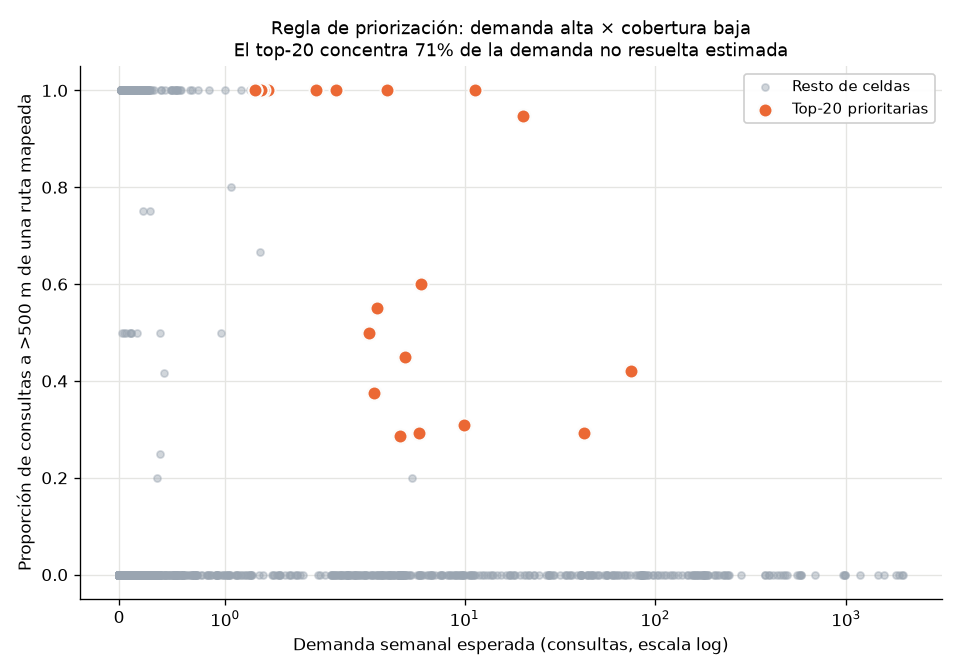
\includegraphics[width=0.75\textwidth]{imagenes/fig_priority_quadrants.png}
  \fuente{Elaboración propia, a partir de \var{27_priority_cells.py} ---
  \var{reports/05_deployment/03_priority_cells.md}.}
\end{figure}

El top-20 de celdas prioritarias concentra el \textbf{70,5~\%} de toda la demanda no resuelta
estimada del área metropolitana. Consistente con la figura, esas celdas \textbf{no son las de
mayor demanda absoluta}: son celdas de demanda baja o media (entre 1 y 74 consultas/semana)
mal cubiertas por el mapeo actual --la misma conclusión de H1 vista desde la decisión
operativa. Dieciocho de las veinte celdas coinciden entre usar Random Forest o la media móvil
como estimador de demanda, coherente con la refutación de la
sección~\ref{sec:sirve-para-priorizar}: el valor de esta tabla está en cruzar demanda con
cobertura, no en el estimador que produce la demanda.

\subsection{Monitoreo y reentrenamiento}
\label{sec:monitoreo}

Los umbrales de monitoreo se derivan de la distribución real de error y volumen de este
proyecto, no de valores convencionales.

\begin{table}[htbp]
  \centering
  \caption{Plan de monitoreo y reentrenamiento}
  \label{tab:monitoreo}
  \interlineadoSimple
  \begin{tabularx}{\textwidth}{@{}p{0.30\textwidth}p{0.16\textwidth}X@{}}
    \toprule
    \textbf{Métrica} & \textbf{Frecuencia} & \textbf{Umbral / acción} \\
    \midrule
    Volumen semanal total de consultas & Semanal & $<10.041$ consultas (30~\% de la mediana
    de las últimas 13 semanas no parciales) $\to$ marcar la semana como incompleta y
    excluirla del cálculo de \texttt{lag1} \\
    MAE semanal (predicción vs. real) & Semanal & $>11{,}64$ consultas (media $+\ 2\sigma$
    de las 6 semanas de prueba limpias) durante 2 semanas consecutivas $\to$ reentrenar antes
    del ciclo trimestral \\
    Actualización del feed GTFS & Semanal & Automática, ya implementada
    (\var{run_update_pipeline.py}) \\
    Reentrenamiento completo & Trimestral & Alineado con la ventana de 13 semanas de la
    validación cruzada (sección~\ref{sec:proceso-entrenamiento}) \\
    \bottomrule
  \end{tabularx}
  \fuente{Elaboración propia, a partir de \var{25_monitoring_plan.py} ---
  \var{reports/05_deployment/02_monitoring_plan.md}.}
\end{table}

El chequeo de completitud de datos existe \emph{porque} la sección~\ref{sec:semanas-parciales}
encontró el problema que previene: con este piso, las semanas 2024-W18 (909 consultas) y
2024-W23 (1.367 consultas) se habrían marcado automáticamente como incompletas en lugar de
descubrirse meses después durante el análisis de errores.

\subsection{Alcance del despliegue y trabajo pendiente}

No se despliega el servicio a un dominio público ni se automatiza el reentrenamiento con un
orquestador real (Airflow o un programador de tareas en un servidor productivo) --fuera del
alcance declarado de este trabajo (capítulo~\ref{cap:alcance}). Lo que se entrega en su lugar
es un prototipo funcional y verificable localmente, una arquitectura documentada que conecta
código ya existente, umbrales de monitoreo cuantificados a partir de los propios resultados
del proyecto, y una limitación operativa real --no hipotética-- descubierta al construir el
prototipo, con su mitigación propuesta. Antes de un uso productivo más allá de lo local
harían falta, como mínimo, autenticación, límites de tasa, un orquestador para el
reentrenamiento periódico y pruebas automatizadas de regresión sobre las métricas del modelo.

